%  LaTeX support: latex@mdpi.com 
%  For support, please attach all files needed for compiling as well as the log file, and specify your operating system, LaTeX version, and LaTeX editor.

%=================================================================
\documentclass[journal,article,submit,moreauthors,pdftex]{Definitions/mdpi} 

% For posting an early version of this manuscript as a preprint, you may use "preprints" as the journal and change "submit" to "accept". The document class line would be, e.g., \documentclass[preprints,article,accept,moreauthors,pdftex]{mdpi}. This is especially recommended for submission to arXiv, where line numbers should be removed before posting. For preprints.org, the editorial staff will make this change immediately prior to posting.

%--------------------
% Class Options:
%--------------------
%----------
% journal
%----------
% Choose between the following MDPI journals:
% acoustics, actuators, addictions, admsci, adolescents, aerospace, agriculture, agriengineering, agronomy, ai, algorithms, allergies, analytica, animals, antibiotics, antibodies, antioxidants, appliedchem, applmech, applmicrobiol, applnano, applsci, arts, asi, atmosphere, atoms, audiolres, automation, axioms, batteries, bdcc, behavsci, beverages, biochem, bioengineering, biologics, biology, biomechanics, biomedicines, biomedinformatics, biomimetics, biomolecules, biophysica, biosensors, biotech, birds, bloods, brainsci, buildings, businesses, cancers, carbon, cardiogenetics, catalysts, cells, ceramics, challenges, chemengineering, chemistry, chemosensors, chemproc, children, civileng, cleantechnol, climate, clinpract, clockssleep, cmd, coatings, colloids, compounds, computation, computers, condensedmatter, conservation, constrmater, cosmetics, crops, cryptography, crystals, curroncol, cyber, dairy, data, dentistry, dermato, dermatopathology, designs, diabetology, diagnostics, digital, disabilities, diseases, diversity, dna, drones, dynamics, earth, ebj, ecologies, econometrics, economies, education, ejihpe, electricity, electrochem, electronicmat, electronics, encyclopedia, endocrines, energies, eng, engproc, entropy, environments, environsciproc, epidemiologia, epigenomes, fermentation, fibers, fire, fishes, fluids, foods, forecasting, forensicsci, forests, fractalfract, fuels, futureinternet, futuretransp, futurepharmacol, futurephys, galaxies, games, gases, gastroent, gastrointestdisord, gels, genealogy, genes, geographies, geohazards, geomatics, geosciences, geotechnics, geriatrics, hazardousmatters, healthcare, hearts, hemato, heritage, highthroughput, histories, horticulturae, humanities, hydrogen, hydrology, hygiene, idr, ijerph, ijfs, ijgi, ijms, ijns, ijtm, ijtpp, immuno, informatics, information, infrastructures, inorganics, insects, instruments, inventions, iot, j, jcdd, jcm, jcp, jcs, jdb, jfb, jfmk, jimaging, jintelligence, jlpea, jmmp, jmp, jmse, jne, jnt, jof, joitmc, jor, journalmedia, jox, jpm, jrfm, jsan, jtaer, jzbg, kidney, land, languages, laws, life, liquids, literature, livers, logistics, lubricants, machines, macromol, magnetism, magnetochemistry, make, marinedrugs, materials, materproc, mathematics, mca, measurements, medicina, medicines, medsci, membranes, metabolites, metals, metrology, micro, microarrays, microbiolres, micromachines, microorganisms, minerals, mining, modelling, molbank, molecules, mps, mti, nanoenergyadv, nanomanufacturing, nanomaterials, ncrna, network, neuroglia, neurolint, neurosci, nitrogen, notspecified, nri, nursrep, nutrients, obesities, oceans, ohbm, onco, oncopathology, optics, oral, organics, osteology, oxygen, parasites, parasitologia, particles, pathogens, pathophysiology, pediatrrep, pharmaceuticals, pharmaceutics, pharmacy, philosophies, photochem, photonics, physchem, physics, physiolsci, plants, plasma, pollutants, polymers, polysaccharides, proceedings, processes, prosthesis, proteomes, psych, psychiatryint, publications, quantumrep, quaternary, qubs, radiation, reactions, recycling, regeneration, religions, remotesensing, reports, reprodmed, resources, risks, robotics, safety, sci, scipharm, sensors, separations, sexes, signals, sinusitis, smartcities, sna, societies, socsci, soilsystems, solids, sports, standards, stats, stresses, surfaces, surgeries, suschem, sustainability, symmetry, systems, taxonomy, technologies, telecom, textiles, thermo, tourismhosp, toxics, toxins, transplantology, traumas, tropicalmed, universe, urbansci, uro, vaccines, vehicles, vetsci, vibration, viruses, vision, water, wevj, women, world 

%---------
% article
%---------
% The default type of manuscript is "article", but can be replaced by: 
% abstract, addendum, article, book, bookreview, briefreport, casereport, comment, commentary, communication, conferenceproceedings, correction, conferencereport, entry, expressionofconcern, extendedabstract, datadescriptor, editorial, essay, erratum, hypothesis, interestingimage, obituary, opinion, projectreport, reply, retraction, review, perspective, protocol, shortnote, studyprotocol, systematicreview, supfile, technicalnote, viewpoint, guidelines, registeredreport, tutorial
% supfile = supplementary materials

%----------
% submit
%----------
% The class option "submit" will be changed to "accept" by the Editorial Office when the paper is accepted. This will only make changes to the frontpage (e.g., the logo of the journal will get visible), the headings, and the copyright information. Also, line numbering will be removed. Journal info and pagination for accepted papers will also be assigned by the Editorial Office.

%------------------
% moreauthors
%------------------
% If there is only one author the class option oneauthor should be used. Otherwise use the class option moreauthors.

%---------
% pdftex
%---------
% The option pdftex is for use with pdfLaTeX. If eps figures are used, remove the option pdftex and use LaTeX and dvi2pdf.

%=================================================================
% MDPI internal commands
\firstpage{1} 
\makeatletter 
\setcounter{page}{\@firstpage} 
\makeatother
\pubvolume{1}
\issuenum{1}
\articlenumber{0}
\pubyear{2021}
\copyrightyear{2020}
%\externaleditor{Academic Editor: Firstname Lastname} % For journal Automation, please change Academic Editor to "Communicated by"
\datereceived{} 
\dateaccepted{} 
\datepublished{} 
\hreflink{https://doi.org/} % If needed use \linebreak
%------------------------------------------------------------------
% The following line should be uncommented if the LaTeX file is uploaded to arXiv.org
%\pdfoutput=1

%=================================================================
% Add packages and commands here. The following packages are loaded in our class file: fontenc, inputenc, calc, indentfirst, fancyhdr, graphicx, epstopdf, lastpage, ifthen, lineno, float, amsmath, setspace, enumitem, mathpazo, booktabs, titlesec, etoolbox, tabto, xcolor, soul, multirow, microtype, tikz, totcount, changepage, paracol, attrib, upgreek, cleveref, amsthm, hyphenat, natbib, hyperref, footmisc, url, geometry, newfloat, caption

%=================================================================
%% Please use the following mathematics environments: Theorem, Lemma, Corollary, Proposition, Characterization, Property, Problem, Example, ExamplesandDefinitions, Hypothesis, Remark, Definition, Notation, Assumption
%% For proofs, please use the proof environment (the amsthm package is loaded by the MDPI class).

%=================================================================
% Full title of the paper (Capitalized)
\Title{Effects of Adversarial Training on the Safety of Classification Models}

% MDPI internal command: Title for citation in the left column
\TitleCitation{Effects of Adversarial Training on the Safety of Classification Models}

% Author Orchid ID: enter ID or remove command
% \newcommand{\orcidauthorA}{0000-0000-0000-000X} % Add \orcidA{} behind the author's name
%\newcommand{\orcidauthorB}{0000-0000-0000-000X} % Add \orcidB{} behind the author's name

% Authors, for the paper (add full first names)
\Author{Handong Kim $^{1}$ and Jongdae Han *}%\orcidA{} and Jongdae Han *}

% MDPI internal command: Authors, for metadata in PDF
\AuthorNames{Handong Kim and Jongdae Han}

% MDPI internal command: Authors, for citation in the left column
\AuthorCitation{Handong Kim., Jongdae Han.}
% If this is a Chicago style journal: Lastname, Firstname, Firstname Lastname, and Firstname Lastname.

% Affiliations / Addresses (Add [1] after \address if there is only one affiliation.)
\address{$^{1}$ \quad Affiliation 1; aggsae@gmail.com}

% Contact information of the corresponding author
\corres{Correspondence: elvenwhite@smu.ac.kr}

% Current address and/or shared authorship
% \firstnote{Current address: Affiliation 3} 
% \secondnote{These authors contributed equally to this work.}
% The commands \thirdnote{} till \eighthnote{} are available for further notes

%\simplesumm{} % Simple summary

%\conference{} % An extended version of a conference paper

% Abstract (Do not insert blank lines, i.e. \\)
\abstract{
Although artificial intelligence(AI) is widely applied in everyday life, requirements other than performance are rarely verified.
In this study, through experiments, we prove that adversarial training can be useful  for early verification of the safety of classification models.
By evaluting the safety of models with adversarial examples of different ratios for datasets and models with three characteristics,
we found that the safety is significantly improved in most cases when adversarial training is performed.
Through the accuracy and safety obtained through evaluations, adversarial training can help models finetune work according to the model requirements.
}

% Keywords
\keyword{Requirements Engineering; Nonfunctional Requirements; Safety; Artificial Intelligence; Adversarial Training;} 

% The fields PACS, MSC, and JEL may be left empty or commented out if not applicable
%\PACS{J0101}
%\MSC{}
%\JEL{}

%%%%%%%%%%%%%%%%%%%%%%%%%%%%%%%%%%%%%%%%%%
% Only for the journal Diversity
%\LSID{\url{http://}}

%%%%%%%%%%%%%%%%%%%%%%%%%%%%%%%%%%%%%%%%%%
% Only for the journal Applied Sciences:
%\featuredapplication{Authors are encouraged to provide a concise description of the specific application or a potential application of the work. This section is not mandatory.}
%%%%%%%%%%%%%%%%%%%%%%%%%%%%%%%%%%%%%%%%%%

%%%%%%%%%%%%%%%%%%%%%%%%%%%%%%%%%%%%%%%%%%
% Only for the journal Data:
%\dataset{DOI number or link to the deposited data set in cases where the data set is published or set to be published separately. If the data set is submitted and will be published as a supplement to this paper in the journal Data, this field will be filled by the editors of the journal. In this case, please make sure to submit the data set as a supplement when entering your manuscript into our manuscript editorial system.}

%\datasetlicense{license under which the data set is made available (CC0, CC-BY, CC-BY-SA, CC-BY-NC, etc.)}

%%%%%%%%%%%%%%%%%%%%%%%%%%%%%%%%%%%%%%%%%%
% Only for the journal Toxins
%\keycontribution{The breakthroughs or highlights of the manuscript. Authors can write one or two sentences to describe the most important part of the paper.}

%%%%%%%%%%%%%%%%%%%%%%%%%%%%%%%%%%%%%%%%%%
% Only for the journal Encyclopedia
% \encyclopediadef{Instead of the abstract}
% \entrylink{The Link to this entry published on the encyclopedia platform.}
%%%%%%%%%%%%%%%%%%%%%%%%%%%%%%%%%%%%%%%%%%
\begin{document}
\section{Introduction}

Software requirements are one of the important factors that affect software quality.
Verifying the requirements in an early stage of software development life cycles helps to more likely develop high-quality software and to save resources that may be needed to resolve future problems.
Requirements can be divided into functional requirements and nonfunctional requirements\_(NFRs).
Functional requirements show whether software properly provides the functions wanted by users, and others are NFRs.
NFRs include the performance\_(whether software performs the desired behavior, accuracy is mainly used), fairness\cite{fairness-microsoft, fairness-dwork, fairness-feldman, fairness-tramer, fairness-zhang, fairness-zemel}, security\cite{security-mei, security-mei2, security-barreno}, safety(whether the execution result of the software is safe)\cite{safety-amodei,safety-juric,safety-leike}, and transparency(whether software can be trusted)\cite{transparency-yosinski,xai-transparency-ribeiro,xai-transparency-murdoch}.
It is essential to verifty not only functional requirements but also NFRs for high-quality software.

Existing software quickly verifies requirements through several methods, such as the V model, which makes detailed documentation and testing at each stage of the software development life cycle.
In existing software, people can directly check the operation of code; thus, functional requirements and NFRs can be verified through codes.

Nevertheless, with the advent of deep neural network and artificial intelligence\_(AI), which has different characteristics from existing common software, it is difficult to verify requirements through methods applied in existing software.
Performance, which is one of the NFRs, can be verified to some extent through accuracy or F1 score measurement. However, other NFRs, such as safety, are difficult to verify.
It is difficult to apply verification methods for existing software in AI because AI operates as a black box model. In existing software, NFRs can be verified through codes, but in AI, it is difficult to verify them because AI cannot identify code operations.
In AI, the verification of NFRs is important, especially in areas that have fatal impacts on humans, such as autonomous driving\cite{ai-driving-bajarski,ai-driving-levinson}, medical diagnosis\cite{ai-medical-ramsundar,ai-medical-vieira,ai-medical-xai-holzinger,ai-medical-krause,ai-medical-tan,ai-medical-pesapane,ai-medical-miller}, and finance\cite{ai-finance-fu}.
If NFRs, such as safety, security, and transparency are not guaranteed, not only fatal human problems but also other problems, such as legal problems about liability may arise.
Nevertheless, quality assessment of AI is mainly performed only on the performance corresponding to how well AI through methods such as accuracy and F1 score, and NFRs have rarely been studied.

Several studies have been conducted in this regard, and such studies can be categorized into two.
The first category directly deals with various types of AI NFRs.

For example:
\begin{itemize}
    \item Studies have defined the fairness of AI, addressed problems that may arise when fairness is not verified, and proposed methods for verifying fairness\cite{fairness-dwork, fairness-feldman, fairness-tramer, fairness-zhang, fairness-zemel}.
    \item In \cite{security-barreno,security-mei,security-mei2}, security problems that can arise due to the vulnerability of AI were defined. Additionally, attack methods that threaten the security of AI and those to prevent them were proposed.
    \item In \cite{transparency-yosinski}, the authors proposed methods for understanding the behavior of AI by visualizing the activation of each layer of the used models.
    \item The authors in \cite{safety-amodei,safety-juric,safety-leike}, defined safety of AI, proposed methods for safety, and the studied previous cases caused by the nonobservance of safety.
\end{itemize}

The second category of studies investigates problmesrelated to the NFRs of AI, although they do not directly address the NFRs of AI.
Explainable AI(XAI) and adversarial training are one of the examples of such of studies.
XAI enables people to understand the process of training and deriving the results of AI.
In other words, it is a process that verifies the transparency AI results\cite{xai-arrieta,xai-samek,xai-transparency-murdoch,xai-transparency-ribeiro,ai-medical-xai-holzinger}.
Advesarial training is the study of making trained models more robust to adversarial examples\cite{adversarial-goodfellow,adversarial-kurakin,adversarial-kurakin2,adversarial-papernot,adversarial-szegedy,adversarial-yuan}.
Although the purpose of these studies is to maintain or improve the performance of models from adversarial examples, it can be interpreted as a verification method to properly classify adversarial examples that threaten the safety of learned models.
Although these studies make some contributions, such as revealing the learning process of models and responding well to adversarial examples, they do not sufficiently contribute to the verification of AI NFRs.
Thus, in this study,on the basis of the above-cited studies, we verify NFRs of AI, especially the \textit{safety} of \textit{classification} models using \textit{adversarial training}.
Among the purposes and NFRs of AI, the reasons for choosing classification and safety and the definition of safety herein will be discussed in more detail in section 3.

In this study, we assume that the safety of classification models can be improved using adversarial examples as a part of data for training(adversarial training).
To prove this, we set up the following research questions(RQs).

\begin{description}
    \item[RQ1.]	Can classification models appropriately classify adversarial examples by adversarial training?
    \item[RQ2.]	Do they show the same results as RQ1 for safety-related datasets?
    \item[RQ3.] Does adversarial training affect safety regardless of the model structure?
    \item[RQ4.]	At what rate will learning with adversarial examples perform the best?
\end{description}

Through experiments to answer each RQ, we obtained the following:

\begin{enumerate}
    \item	Adversarial training can improve safety performance. Depending on the experimental results, safety is improved by 20\%--40\%.
    \item	Adversarial training can be verified for the safety of AI. Experimental results show that adversarial training can affect safety improvement, which can be a verification method to ensure safety by pregenerating and using adversarial examples.
    \item   Adversarial training can be utilized as a factor to verify safety regardless of the model structure. Similar results have been observed between experiemntal and numerical results, regardless Of the model structure.
    \item	Herein, We propose a process of adjusting the ratio of inclusion adversarial examples in training datasets according to the preferential requirements. Experimental results with different adversarial example inclusion ratios show that adversarial inclusion ratios play key roles in a tradeoff between accuracy and safety.
\end{enumerate} 

The rest of this paper is structured as follows. In section 2, we review previous studies on verification methods for AI NFRs.
In section 3, we define the safety and experimental designs applied in this study.
In section 4, we reports experiments conducted according to the designed experimental methods, and we analyze and discuss the experiemntal results in section 5.
We conclude the paper and recommend future work in section 6.

%%%%%%%%%%%%%%%%%%%%%%%%%%%%%%%%%%%%%%%%%%
\section{Related work}

Prior studies have directly and indirectly addressed the NFRs verification of AI.

\subsection{Studies that directly addressed the NFRs of AI}

\subsubsection{Fairness of AI}

AI learns the features of data and derives the results of input data based on the learned features.
Because of these characteristics, if there is a bias in the training dataset, discriminatory results are obtained for each individual or group using AI.
Such results do not satisfying fairness, an AI NFR that requires every user to achieve the same results.
As reported in \cite{fairness-dwork, fairness-zemel}, bias in training datasets can lead to discriminatory results according to features such as race, gender, and age of each individual.
To solve this problem, the authors proposed a statistical method to identify the discriminating elements of training datasets, argued that it is important to keep the fairness of AI as data bias is related to privacy.
Authors in \cite{fairness-feldman} proposed the problem of discrimination that discriminatory features of datasets can have on groups using AI and a method to solve such a problem.
Additionally, \cite{fairness-zhang} showed that the imbalance of not only data but also data features can affect the performance of AI.
To improve the fairness of AI, \cite{fairness-feldman,fairness-microsoft, fairness-tramer} ensured the fairness of AI by removing or finding factors, such as bias in datasets.

\subsubsection{Security of AI}

The field of application of AI has been expanded to areas closely related to human privacy.
The more AI is applied to private fields, the more it demands security for sensitive information, such as personal information.
Studies have been conducted to identify and classify various security problems occurring because of vulnerabilities in AI and attacks that can cause security problems\cite{security-barreno}.
There are studies that suggest attack methods that can threaten security through these vulnerabilites and defense methods to defend them.
Authors in \cite{security-mei2} proposed the attack method that can threaten the security against tools widely used in actual data analysis.
Authors in \cite{security-mei} proposed the methods to attack security through attacks on training data and the contents of maintaining the security by defending the methods.

\subsubsection{Transparency of AI}

Most of the AI currently applied to operate in black box, users couldn't identify what process the results were derived from models.
Lack of transparency in AI due to black box operations can lead to several complex issues, including legal issues regarding who is responsible when problems arise due to AI's decisions.
Authors in \cite{transparency-yosinski} proposed two tools to visualize layers activated in the process of deriving results for convolutional network-based machine and deep learning models.
By confirming visualized active layers, users can check whether the corresponding result is accurately derived and prevent problems caused by wrong decisions in advance.

\subsubsection{Safety of AI}

According to the dictionary, safety is "a state in which or a place where you are safe and not in danger or at risk.".
If AI, the decision of AI does not pose any danger or risks to humans who apply it in many other fields.
This is important in areas, such as autonomous driving, where AI decisions have a significant impact on humans, just like security.
This is because if safety is not properly verified, it can lead to casualties beyond just damage.
Safety issues that occur in existing AI studies have been addressed\cite{safety-amodei}.
Case analysis has shown that high-performance techniques can lead to safety problems due to other side effects.
Authors in \cite{safety-juric,safety-leike} described the concept and definition of safety in AI and proposed methods for achieving safety.

\subsection{Studies that indirectly addressed NFRs of AI}

In the previous section, we reviewed studies that directly addressed NFRs of AI.
Besides such studies, some studies addressed NFRs of AI in other studies.
For example, XAI and adversarial training are related to transparency and safety, respectively.
In this section, we investigate XAI and adversarial training and how they indirectly address NFRs of AI.

\subsubsection{Explainable AI}

The main purpose of the studies conducted on XAI is not to verify AI NFRs.
However, such studies have revealed the learning and result derivation process in AI, which is directly related to the transparency of AI. Therefore, such studies are considered as related studies.
A characteristic of AI is that it works in a black box: people cannot check what features AI learns from training data and what process it goes through to derive results.
Hence, the derived results cannot be trusted unconditionally.
Particularly, it is more important to solve these problems in fields where results have a large impact on humans, such as autonomous driving and medical diagnosis.
To solve this problem, XAI applied to enable humans to check the AI learning process and that through which results.
Some studies have defined the concept of XAI and introduced the methodology used for XAI to organize previous studies on XAI\cite{xai-samek, xai-arrieta,ai-medical-xai-holzinger,xai-transparency-ribeiro,xai-transparency-murdoch} .

\subsubsection{Adversarial examples and attacks}

The main purpose of studies conducted on adversarial examples and training is not to verify AI NFRs.

However, in \cite{adversarial-kurakin}, it was noted that
\begin{quote}
   "a good response to adversarial examples is an important safety issue in AI."
\end{quote}
Therefore, adversarial examples are related to the safety of AI.

Previous studies have shown that the characteristics of AI learning algorithms are vulnerable to adversarial examples, which behave as adversarial examples regardless of the structure and training data of the models\cite{adversarial-szegedy,adversarial-goodfellow}.
Authors in \cite{adversarial-goodfellow} proposed a fast gradient sign method(FGSM) that uses gradients from the learning process to generate adversarial examples.
Authors in \cite{adversarial-kurakin2} demonstrated through experiments that when the original data used for learning are captured using a smartphone camera and applied to the model, they behave like an adversarial examples. It is effective in real environments rather than experimental environments.
Authors in \cite{adversarial-papernot} proposed a method for adversarial attacks in a black box environment, with no information regarding the network the training dataset, rather than the existing white box approach in which the structure of the etwork and training dataset is known.
Authors in \cite{adversarial-yuan} summarized and classified methods for generating adversarial examples that have been recently addressed.

Several studies on NFRs have been reported, and even in studies that do not primarily consider NFRs, attributes related to the verification of NFRs can be confirmed.
Inspired by these cited studies, we conducted this study.

%%%%%%%%%%%%%%%%%%%%%%%%%%%%%%%%%%%%%%%%%%
\section{Overview of our works}

In this section, we define safety and present an overview of experiments to prove our established RQs.

\subsection{Definition of safety}

AI must ensure minimum safety regardless of its purpose. In a field where AI is applied, the actual input data may not exist in the dataset used for training.
Additionally, AI suffers from multiple threats in real-world applications, such as adversarial attacks(adversarial examples).

\begin{figure}[H]
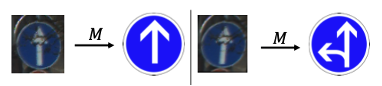
\includegraphics[width=13 cm]{Definitions/example-of-adversarial.png}
\caption{Examples of adversarial examples.\label{example-of-adversarial}}
\end{figure}   

Examples of adversarial attacks are shown in Figure~\ref{example-of-adversarial}. Both signs appear the same sign in human eyes. Nevertheless, the right one with an adversarial attack is not properly classified compared with the left one.
Models applied to fields where the results can have significant impacts on humans, such as autonomous driving and medical diagnosis, can cause fatal safety problems if they do not properly respond to adversarial attacks. Thus, in such a field, it is important to respond well to adversarial attacks and ensure safety.
Based on this, herein, we define safety as

\begin{quote}
    "a measure of whether a model responds appropriately to data with untrained features or to data that have been adversarially attacked to obtain incorrect results from the model."
\end{quote}

Learning all data and adversarial examples that may occur in an environment in which the model is applied is the best way to ensure safety.
However, in reality, it is difficult to collect all data in all situations, and even if they are collected, a lot of resources are consumed to process and train them.
Therefore, in a situation where all data cannot be learned, which data should be learned first to ensure minimum safety?

\subsection{Overview of our experiments}

Herein, we assume that adversarial examples are given the highest priority and are the data that should be learned.
This is because adversarial examples are data designed to cause problems or confuse the results of the model.
For data under other conditions, the results derived from the model unconditionally cause problems.
Conversely, adversarial examples are likely to cause problems with the model's results.
For example, in traffic signs for autonomous driving, there may be data to cause problems, as shown in Figure~\ref{example-of-adversarial}, whereas there may be data that do not necessarily cause problems, such as traffic signs with natural environments(sunlight, fog, etc.).
Another reason is the difficulty in creating and configuring datasets. Generating corresponding data is difficult because there are too many conditions for the data that can occur in the environment in which the model is applied.
Conversely, in the case of adversarial examples, several studies on adversarial attack methods for this purpose have been conducted. Therefore, it is relatively easy to generate when compared with the previous data.
For these reasons, adversarial training can be a way to ensure minimum AI safety, which has been proven through experiments.
If adversarial training allows a model to better respond to adversarial examples, i.e., to improves safety performance, it can be used to verify whether safety is guaranteed in advance by preparing adversarial examples before training and mixing them with the training data.

To show this through experiments, we first prepared different kinds of dataset and used them to generate adversarial datasets with different degrees of transformation \begin{math}\epsilon\end{math}.
Several degrees of \begin{math}\epsilon\end{math} were prepared to check the effect of \begin{math}\epsilon\end{math} on safety performance. If \begin{math}\epsilon\end{math} is too small, the safety performance will not improve because there is little difference from the original data. Thus, it cannot classify adversarial examples well. If it(\begin{math}\epsilon\end{math}) is too large, the features of the original data cannot be learned properly, resulting in a poor performance like the accuracy of the existing model.
Additionally, when generating datasets for adversarial training, the size of the training dataset was maintained the same as the size of the existing training dataset.
This is because increasing the number of data does not necessarily improve the performance of the model and requires additional resources to learn them.
Furthermore, to show at what ratio adversarial examples should be included for safety verification in the data preparation stage, an experiment was conducted by setting the mixing ratio of the original data and the adversarial examples differently.
Then, when adversarial training was executed, the number of original training data was reduced, thus, the accuracy, which is one of the performance evaluation measures of the model for accurately classifying the original evaluation dataset, may decrease\cite{trade-off}. 
It is important to improve safety, but accuracy can be more important in some cases, depending on the purpose of the model.
Therefore, it is necessary to ensure accuracy and safety. 
Thus, in order to maintain the accuracy of the model learned with the original dataset and appropriate resources, we mixed the original data and adversarial examples at an appropriate ratio while preserving the size of the training dataset.
To show this, accuracy is selected as an additional measure for performance evaluation.
Although both accuracy and safety are measures for classifying a given data we divided the measures by the target evaluation dataset to distinguish them on a scale with different meanings.
Accuracy represents how well a model classifies the {\it original} evaluation dataset, and safety represents how well model classifies the {\it adversarial} evaluation dataset, which is considered threatening to the model according to the definition given above.
With the belief that results may differ according to the characteristics of the model's structure, we prepared learning models with different structures. 
Detailed informations regarding the dataset, adversarial attack method, accuracy, safety, models, and experimental methods are discussed in section 4.

%%%%%%%%%%%%%%%%%%%%%%%%%%%%%%%%%%%%%%%%%%
\section{Methodology}

We conducted experiments under different conditions to answer the formulated RQs. For the experiment, we prepared a dataset with three characteristics and models with three structures.
Section 4.1 introduces the dataset and models used in our experiment and the reason they were selected.
Section 4.2 presents a brief introduction to FGSM for generating adversarial examples and the reason it is was selected.
Section 4.3 introduces each experimental process designed in section 3.

\subsection{Datasets and Models}

\subsubsection{Datasets}

For the experiments, three datasets, including CIFAR-10, CIFAR-100\cite{cifar}, and German traffic sign recognition benchmark(GTSRB)\cite{gtsrb}, were used.
CIFAR-10 comprises 60,000 data in 10 classes, each containing 6,000 data with three channels and \begin{math}{32\times 32}\end{math} in size.
Among these, 5,000 data were used for training, and the remaining were used for evaluation.

\begin{figure}[H] 
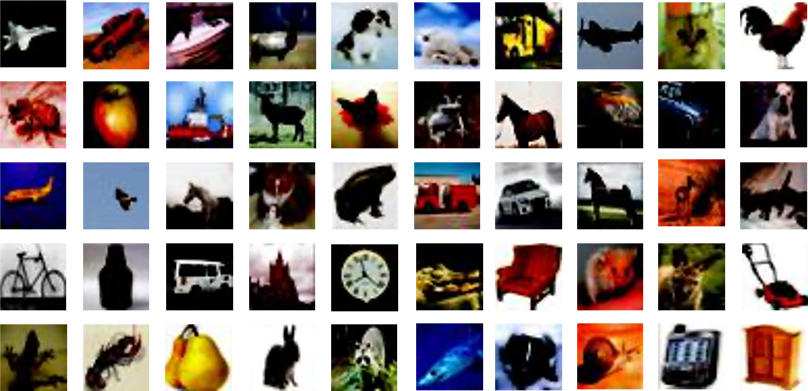
\includegraphics[width=13cm]{Definitions/cifar-datasets.png}
\caption{CIFAR datasets.\label{cifar-datasets}}
\end{figure} 

Figure~\ref{cifar-datasets} shows some CIFAR datasets.
CIFAR-100 ccomprises 60,000 data in 100 classes, each class containing 600 data with three channels and \begin{math}{32\times 32}\end{math} in size. Among them, 500 data were used for training, and the remaining were used for evaluation.
CIFAR-10 and CIFAR-100 were used for the experiment to answer RQ1, which corresponds to the most basic hypothesis established herein.
This is due to the difference between CIFAR-10 and CIFAR-100. CIFAR-10 has a large number of data for small classes, which is likely for the model to learn features for each class.
Conversely, CIFAR-100 has a small number of data for many classes, so the model is less likely to learn features for each class.
If it is possible to identify the improvement of safety through adversarial training for datasets with these opposite characteristics, valid results can be seen for most training datasets with characteristics intermediate between CIFAR-10 and CIFAR-100. Thus, we used CIFAR datasets for the experiment.

\begin{figure}[H]
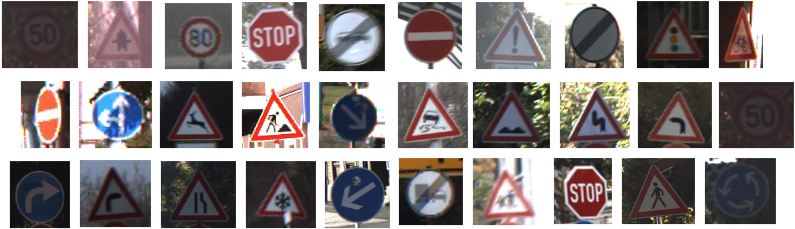
\includegraphics[width=13 cm]{Definitions/gtsrb-dataset.png}
\caption{GTSRB.\label{gtsrb-dataset}}
\end{figure} 

The German Traffic Sign Recognition Benchmark GTSRGB is a German traffic sign dataset. It comprises more than 50,000 data under 43 classes.
The difference between GTSRB and CIFAR datasets is the number of data corresponding to each class.
Figure~\ref{gtsrb-dataset} shows some GTSRB data.
The dataset used for applicable AI training has some of this data bias.
Thus, we selected GTSRB because we assume if it is possible to identify the safety improvement of a model through adversarial training for datasets in which the number of data is not uniform for each class, we can get valid results for other datasets.
Another reason for selecting GTSRB is that it is closely related to safety.

\subsubsection{Models}

Herein, three models with different structures were applied to understand the effect of adversarial training through data augmentation on safety performance regardless of the network structure.
LeNet\cite{lenet} is a classical convolutional neural network-structured model developed in 1998 and features better performance when compared when its simple structure.
LeNet has the simplest structure among the models used in the experiment herein. It was used to understand the effect of simple structured model.
ResNet18\cite{resnet} and VGG16\cite{vgg} are the most well-known and widely used models for classification, and their performance has also been proven through ImageNet large scale visual recognition challenge.
Although VGG16 came second in the 2014 competition, it is more popular than the winning model GoogLeNet because of its simplicity and ease of use.
ResNet18 won the 2015 competition with the addition of Residual blocks to VGGNet.
Herein, we selected two models with guaranteed classification performance through the competition prize for experiments.
ResNet18 was chosen because it has a complex structure, and VGG16 has a structure intermediate between ResNet18 and LeNet.
For LeNet, we directly implemented the model by referring to the paper and used it.
For ResNet18 and VGG16, models defined in {\it "torchvision.models"} of PyTorch\cite{pytorch}, one of the deep learning frameworks used for Python, were used.
The models were not separately finetuned, and the rest of the hyperparameters were used under the same conditions, except for epoch.
The same conditions were set without additional adjustment because we did not consider models producing optimal performance.
Moreover, adjusting the model structure and hyperparameters can result in better performance through multiple training and evaluation processes, but it needs several resources and does not help much for AI safety.
However, for the epoch, the accuracy exceeded 90\% in training within the maximum range of 30. This is because the structures of the used models are different; hence, when experiments were conducted with the same epoch, overfitting occurred in some models.

\subsection{FGSM}

We assume that the safety of AI is how well it classifies adversarial examples mentioned in section 3.
Hence, it is necessary to generate adversarial examples. Among several adversarial attack methods to generate adversarial examples, we used FGSM\cite{adversarial-goodfellow}.
Because FGSM generates adversarial examples using gradient in the training process, it is necessary to train at least once with the dataset that we want to generate adversarial examples.
Thus, to generate adversarial examples, we used LeNet, which has a relatively simple structure and does not require much time to learn in our paper.

\begin{figure}[H] 
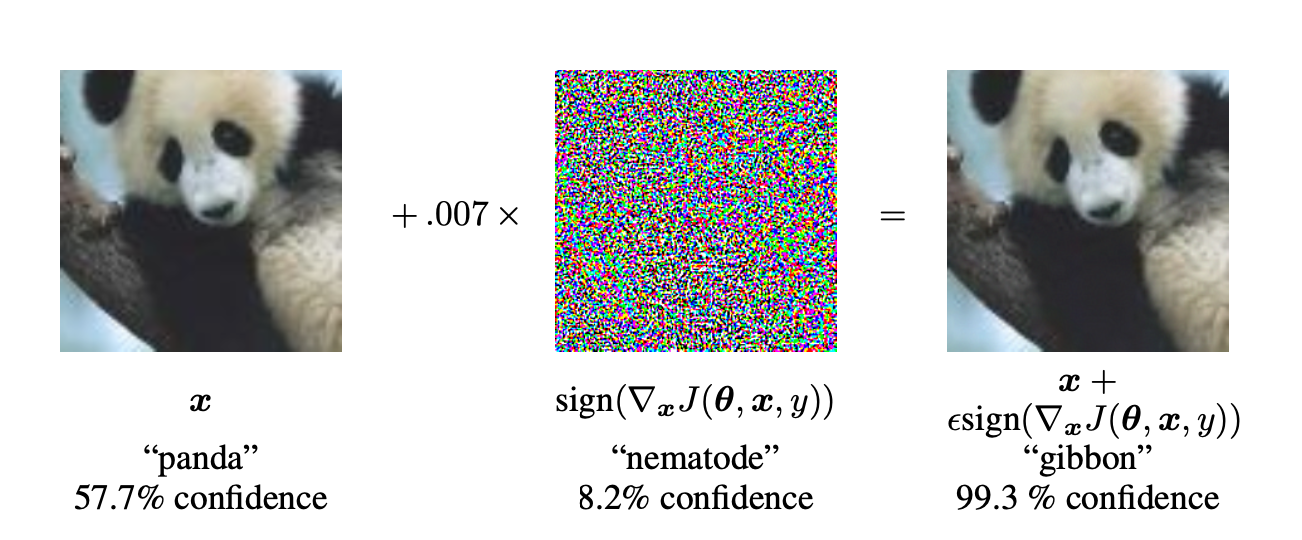
\includegraphics[width=13cm]{Definitions/fgsm.png}
\caption{Process of generating adversarial examples with FGSM. Image adapted from \cite{adversarial-goodfellow}\label{fgsm}}
\end{figure} 

As shown in Figure~\ref{fgsm}, adversarial examples were generated using the gradient change that occuring during the training process.
At this time, \begin{math}\epsilon\end{math} was used to determine the degree of adversarial attack by reflecting the slope value.
Herein, 0.05 and 0.1 were used as \begin{math}\epsilon\end{math}. Failure to use values above 0.1 is due to the observation of human-observable transformation points in adversarial examples.
Thus, if the value is greater than 0.1, it can no longer serve as an adversarial example. Therefore, two types of \begin{math}\epsilon\end{math} are used to generate adversarial examples.
In \cite{adversarial-goodfellow}, adversarial examples were applied only to the evaluation data to confirm the effect of adversarial examples. Nevertheless, herein, the training data were also to create adversarial examples because adversarial examples should be used for training.

\begin{figure}[H]
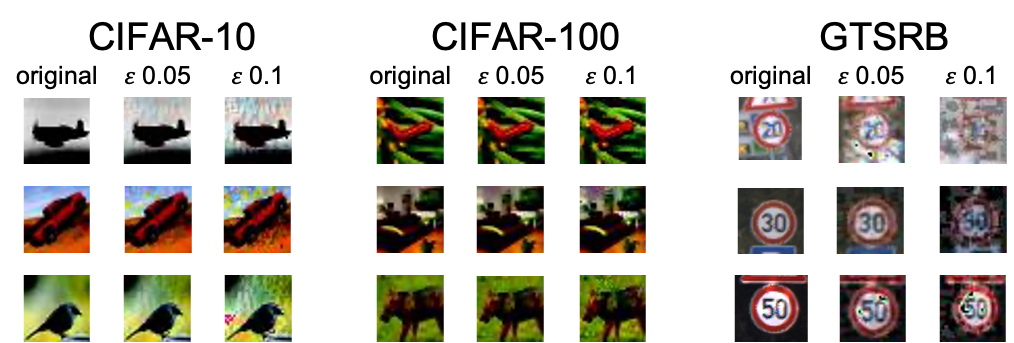
\includegraphics[width=13 cm]{Definitions/adversarial-dataset.png}
\caption{Examples of adversarial examples.\label{adversarial-examples}}
\end{figure} 

Through this method, as shown in Figure~\ref{adversarial-examples}, adversarial examples were generated for all CIFAR-10, CIFAR-100, and GTSRB data to be used for experiments.
In this paper, the training and evaluation data, to which the adversarial attack is applied, are referred to as {\it adversarial training} and {\it evaluation data}.
The generated adversarial training data were randomly extracted at a certain ratio and mixed with the original training data to be used for training, and the adversarial evaluation data were used for experiments to evaluate the safety.

\subsection{Methodology}

We conducted the experiments using a PC with Ubuntu 18.04 OS, 4.20GHz Intel(R) i7-7700K CPU, 64GB RAM, and NVIDIA Titan XP 12GB GPU.

The models used in the experiment have hyperparameters set to a batch size of 64, a learning rate of 0.001, a momentum of 0.9, CrossEntropy as loss functions, and SGD as optimization functions.

Figure~\ref{methodology} shows picture of the experimental procedure.

\begin{figure}[H]
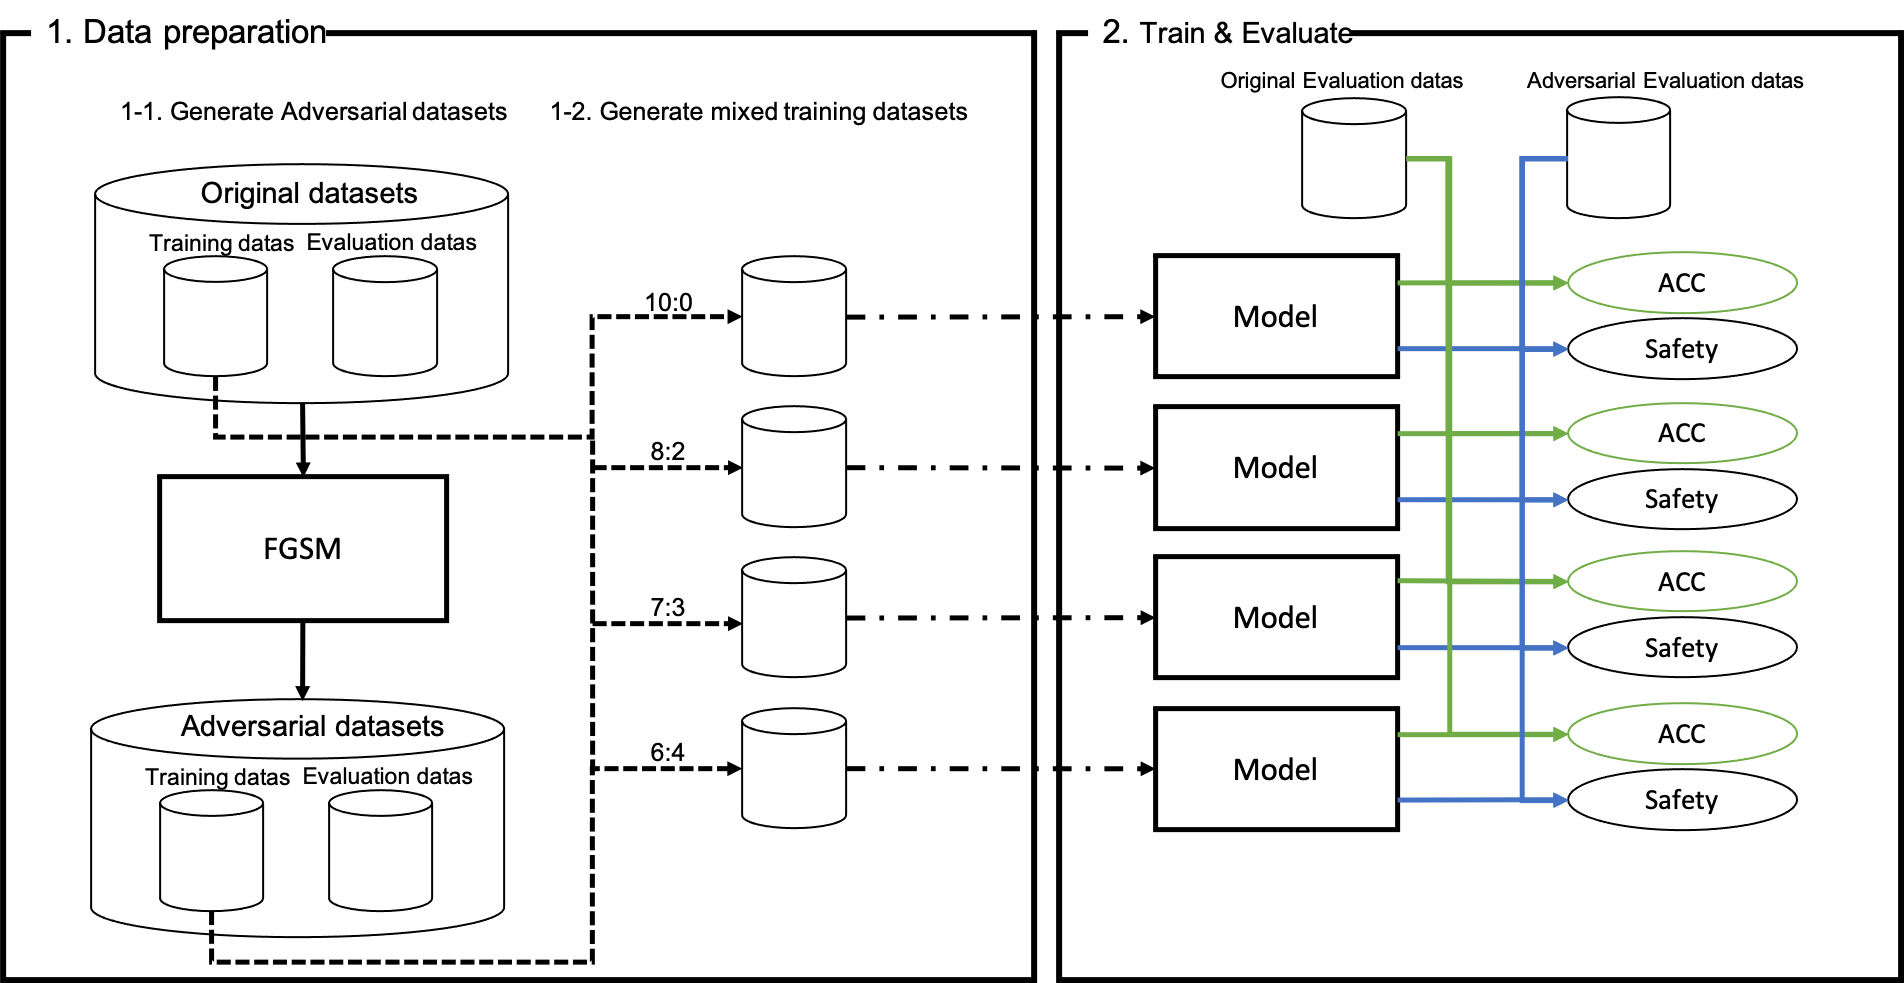
\includegraphics[width=13 cm]{Definitions/methodology.png}
\caption{Experimental procedure\label{methodology}}
\end{figure} 

The experiment was mainly divided into two stages.
The first step was data preparation. 
We generated the adversarial dataset by applying FGSM in 4.2 to the original dataset.
At this time, the adversarial attack was applied not only to both the evalutation data and training data.
The generated adversarial training data were subjected to one more process data mixing process.
We generated mixed training data by randomly extracting the data from the original training data and the adversarial training data according to the specified ratio while preserving the total number of training data the same as the total number of original training data.
At this time, from mixing ratios were used(Figure~\ref{methodology} 1-2).
The mixed training data, original evaluation data, and adversarial data generated through this step were used in the model training and evaluation step.

The second step involves training and evaluating the models.
The mixed training data generated in the previous step was used for training.
Using the mixed training data for the model set with the aforementioned hyperparameters, the training proceeded to the epoch in which the accuracy measured during the training process exceeded 90\%.
If the training accuracy does not reach 90\% until the 30 epoch is reached, the 30 epoch model is used for evaluation.
The trained model evaluates the accuracy and safety using the original evaluation and the adversarial evaluation data, respectively.

%%%%%%%%%%%%%%%%%%%%%%%%%%%%%%%%%%%%%%%%%%
\section{Experimental Results and Discussions}

We hypothesized that adversarial training can significantly improve safety while minimizing the impact on performance, and we designed experiments to verify the assumptions.
This section summarizes and discusses the results of the designed experiments.
Before discussing the experimental results, we define some words in this section.
First, a dataset without any adversarial examples, is called {\it orig}. The training data and evaluation data in {\it orig} are called {\it orig\_train} and {\it orig\_eval}, respectively.
A dataset with adversarial examples, is called {\it adv}, and the training data and evaluation data in {\it adv} are called {\it adv\_train} and {\it adv\_eval}, respectively.
These refer to each dataset and the number of data contained in each dataset.
The {\it N-model} is a model trained on mixed training data containing N\% of the total number of training data with adversarial examples.
For example, a model trained without any adversarial training data is called 0-model, and a model trained with mixed train data containing 20\% of the number of adversarial training data is called 20-model.
{\it N-model} evaluates each evaluation data. The, the number of all correctly classified data is expressed by adding {\it correct} in front of each evaluation data.
For example, if the evaluation data are {\it orig\_eval}, the number of all correctly classified data is termed {\it correct\_orig\_eval}, and if evaluation data are {\it adv\_eval}, the number of all correctly classified data is termed {\it correct\_adv\_eval}.

We used accuracy and safety to evaluate the experimental results. Accuracy is a measure of how well the trained model classifies {\it orig\_eval} and can be expressed as follows:

\begin{equation}
    acc(\%) = \text{{\it correct\_orig\_eval}} / \text{{\it orig\_eval}} \times 100
\end{equation} 

Safety is a measure of how well the trained model classifies {\it adv\_eval}, and it can be expressed as follows:

\begin{equation}
    safety(\%) = \text{{\it correct\_adv\_eval}} / \text{{\it adv\_eval}} \times 100
\end{equation}

Although the same equation is applied, we distinguish between the two parameters depending on whether the evaluation data are in {\it orig\_eval} or {\it adv\_eval}.

\subsection{CIFAR-10 Results}

\begin{specialtable}[H]
    \centering
    \caption{Results of CIFAR-10 with \begin{math}\epsilon\end{math}}
    \label{cifar10-result}
    {\small
    \begin{tabular}{|c|c|c|c|c|c|c|c|}
    \hline
    \multirow{2}{*}{Mixed ratio} & \multirow{2}{*}{Matrix} & \multicolumn{3}{c|}{\begin{math}\epsilon=\end{math}0.05}            & \multicolumn{3}{c|}{\begin{math}\epsilon=\end{math} 0.1}         \\ \cline{3-8} 
                                 &                           & LeNet               & ResNet18              & VGG16              & LeNet              & ResNet18              & VGG16              \\ \hline
    \multirow{2}{*}{10:0}        & Acc                       & 63                  & 53                    & 78                 & 63                 & 53                    & 78                 \\ \cline{2-8} 
                                 & Safety                    & 18                  & 33                    & 33                 & 11                 & 27                    & 27                 \\ \hline
    \multirow{2}{*}{8:2}         & Acc                       & 60                  & 51                    & 73                 & 60                 & 50                    & 74                 \\ \cline{2-8} 
                                 & Safety                    & 45                  & 35                    & 56                 & 38                 & 31                    & 53                 \\ \hline
    \multirow{2}{*}{7:3}         & Acc                       & 58                  & 49                    & 72                 & 57                 & 49                    & 69                 \\ \cline{2-8} 
                                 & Safety                    & 45                  & 36                    & 56                 & 41                 & 34                    & 54                 \\ \hline
    \multirow{2}{*}{6:4}         & Acc                       & 58                  & 48                    & 70                 & 58                 & 47                    & 70                 \\ \cline{2-8} 
                                 & Safety                    & 47                  & 36                    & 56                 & 45                 & 34                    & 56                 \\ \hline
    \end{tabular}
    }
\end{specialtable}

Table~\ref{cifar10-result} lists the CIFAR-10 results according to \begin{math}\epsilon\end{math} for each model.

The results for the adversarial examples produced with \begin{math}\epsilon\end{math} of 0.05 show significant accuracy and safety, with 45\%  in LeNet, 20\% in ResNet18, and 45\% in VGG16.
The 0-model and 20-model showed a decrease in accuracy by 3\%(LeNet), 2\%(ResNet18), and 5\%(VGG16) for each model, but in the case of safety, it was improved by 27\%(LeNet), 2\%(ResNet18), and 23\%(VGG16) for each model.
Although there is a difference between the 30-model and 40-model, the accuracy slightly decreased compared with that of 0-model, and the safety was significantly improved.
Comparing the 20-model, 30-model, and 40-model, lower accuracy and higher safety were confirmed in the model with a high proportion of adversarial examples, but the differences were not large.
In the results for the adversarial examples produced with \begin{math}\epsilon\end{math} of 0.1, as in \begin{math}\epsilon\end{math} of 0.05, the accuracy of the 20-, 30-, 40-model was slightly reduced when compared with the 0-model, but the safety was significantly improved.

\begin{figure}[H]
    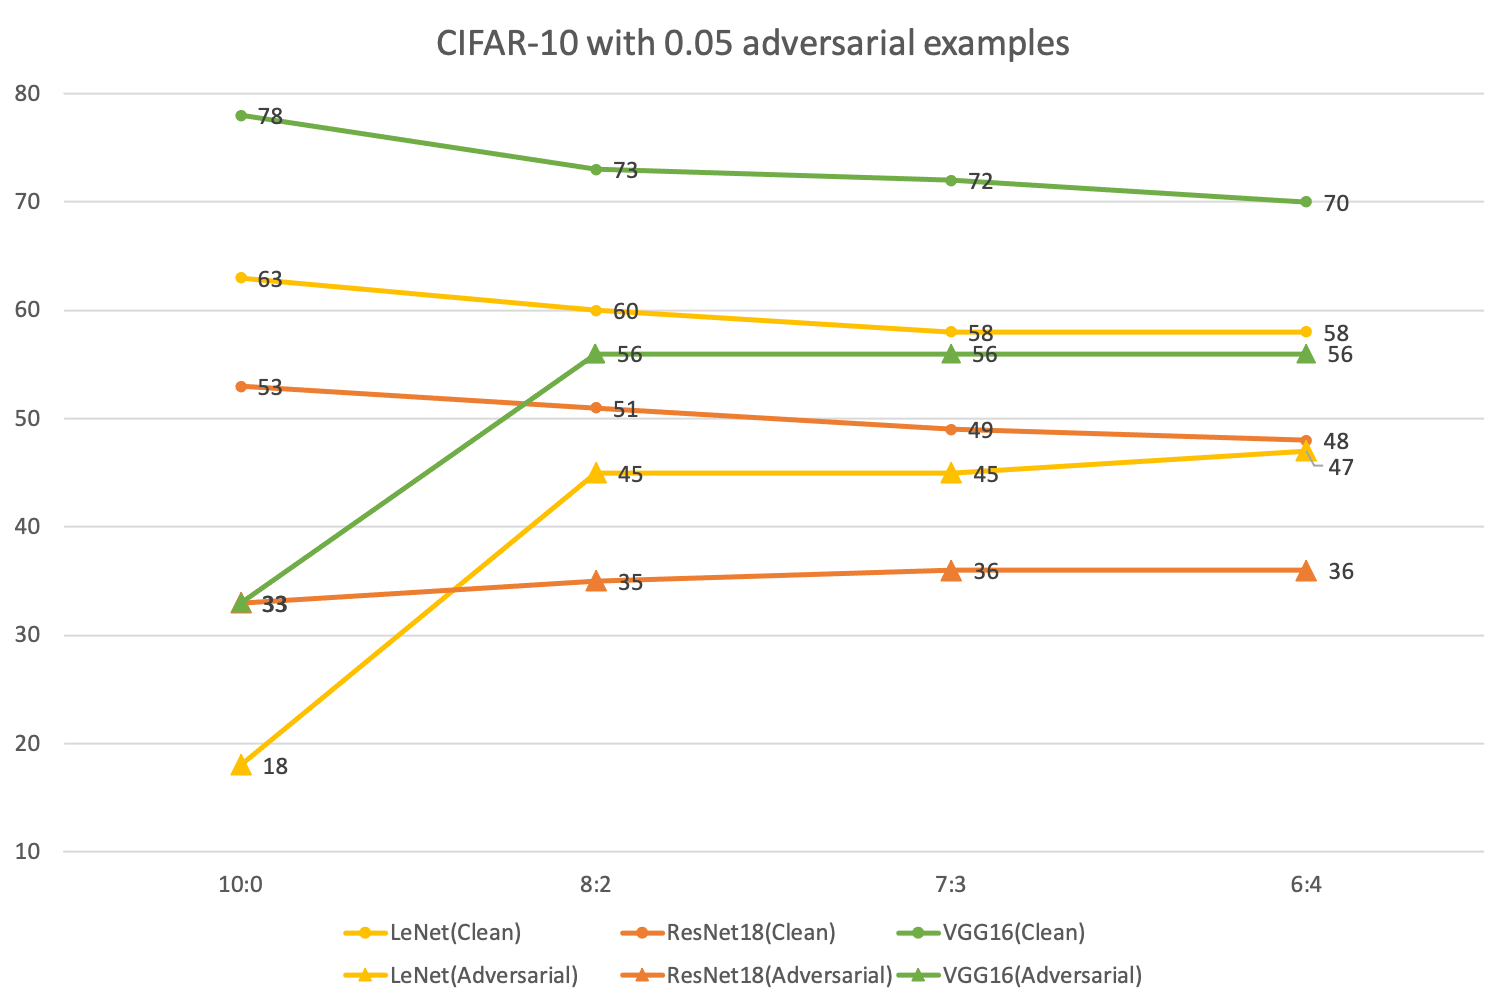
\includegraphics[width=13 cm]{Definitions/graph-005cifar10.png}
    \caption{Graphs of CIFAR-10 with \begin{math}\epsilon\end{math} of 0.05\label{cifar10-0.05-graph}}
\end{figure}

These results are shown in Figure~\ref{cifar10-0.05-graph} and Figure~\ref{cifar10-0.1-graph}, which graphically illustrated the Table~\ref{cifar10-result}.
Figure~\ref{cifar10-0.05-graph} confirms the results for {\it adv\_eval} with \begin{math}\epsilon\end{math} of 0.05.
As shown in Table~\ref{cifar10-result}, when adversarial examples were included at a higher rate, the accuracy was slightly decreased, but the safety was greatly improved.

\begin{figure}[H]
    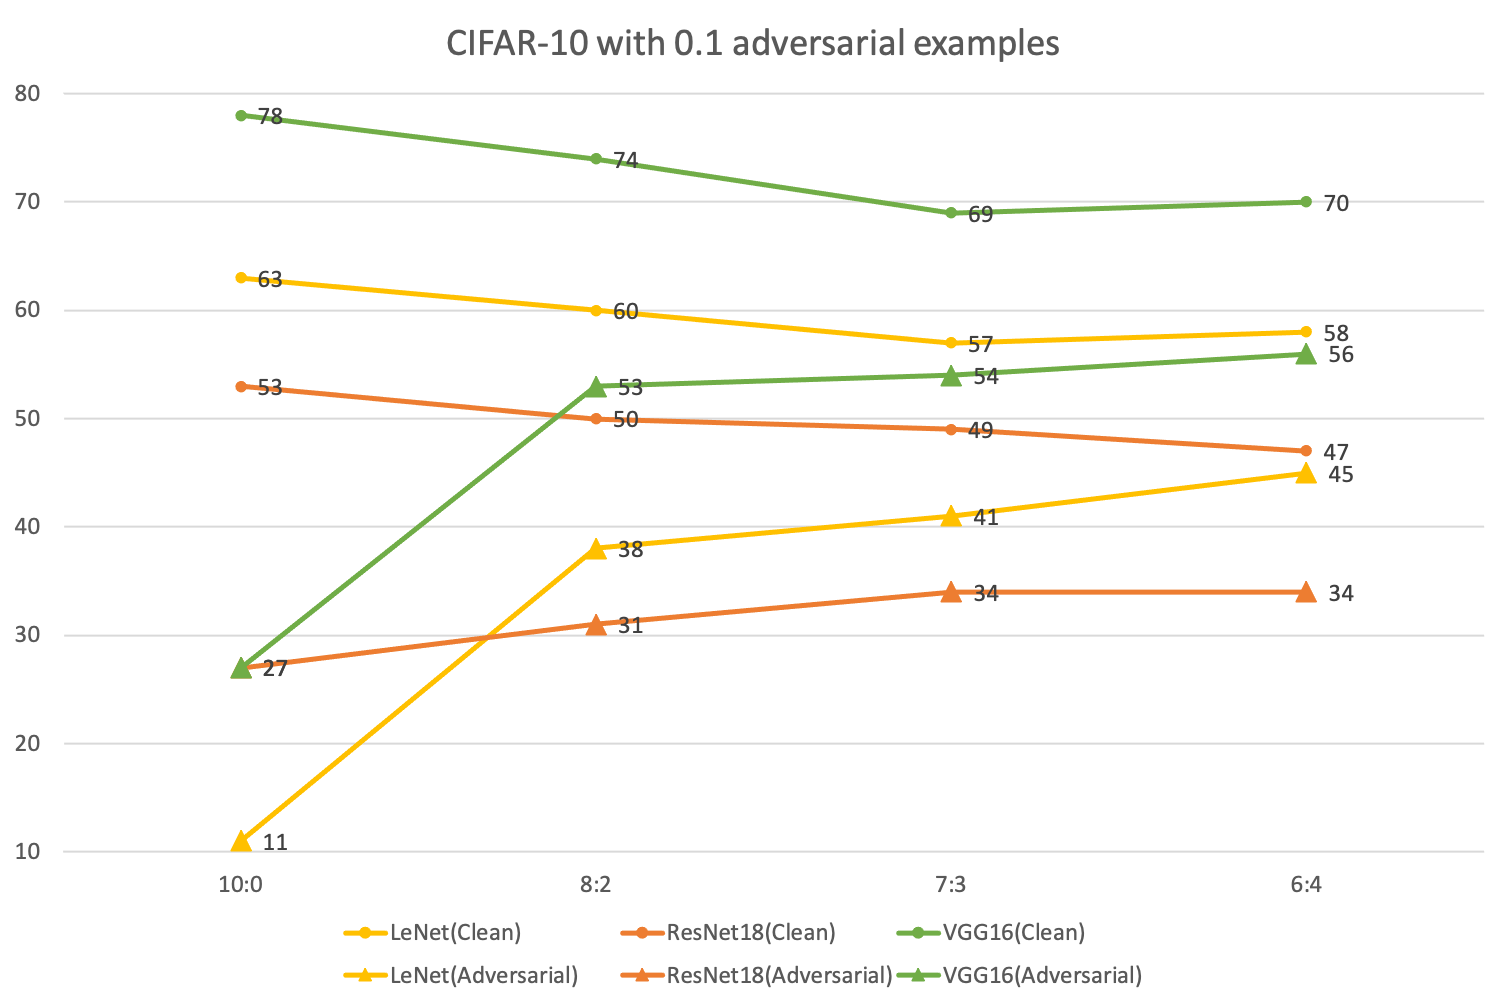
\includegraphics[width=13 cm]{Definitions/graph-01cifar10.png}
    \caption{Graphs of CIFAR-10 with \begin{math}\epsilon\end{math} of 0.1\label{cifar10-0.1-graph}}
\end{figure}

Figure~\ref{cifar10-0.1-graph} shows the results for {\it adv\_eval} made with \begin{math}\epsilon\end{math} of 0.1.
Similar to Figure~\ref{cifar10-0.05-graph}, the accuracy and safety change as the ratio of containing adversarial examples increases.

\subsection{CIFAR-100 Results}

\begin{specialtable}[H]
    \centering
    \caption{Results of CIFAR-100 with \begin{math}\epsilon\end{math}}
    \label{cifar100-results}
    {\small
    \begin{tabular}{|c|c|c|c|c|c|c|c|c|}
    \hline
    \multirow{2}{*}{Mixed ratio} & \multirow{2}{*}{Matrix} & \multicolumn{3}{c|}{\begin{math}\epsilon=\end{math} 0.05}  & \multicolumn{3}{c|}{\begin{math}\epsilon=\end{math} 0.1}       \\ \cline{3-8}
                                 &                           & LeNet               & ResNet18              & VGG16       & LeNet              & ResNet18              & VGG16              \\ \hline 
    \multirow{2}{*}{10:0}        & Acc                       & 27                  & 19                    & 40          & 27                 & 19                    & 40                 \\ \cline{2-8} 
                                 & Safety                    & 15                  & 7                     & 10          & 4                  & 6                     & 7                  \\ \hline 
    \multirow{2}{*}{8:2}         & Acc                       & 26                  & 17                    & 33          & 25                 & 17                    & 35                 \\ \cline{2-8} 
                                 & Safety                    & 15                  & 9                     & 20          & 12                 & 8                     & 21                 \\ \hline 
    \multirow{2}{*}{7:3}         & Acc                       & 26                  & 17                    & 33          & 21                 & 16                    & 29                 \\ \cline{2-8} 
                                 & Safety                    & 15                  & 10                    & 22          & 12                 & 9                     & 20                 \\ \hline 
    \multirow{2}{*}{6:4}         & Acc                       & 24                  & 15                    & 30          & 22                 & 16                    & 26                 \\ \cline{2-8} 
                                 & Safety                    & 18                  & 10                    & 22          & 15                 & 10                    & 20                 \\ \hline 
    \end{tabular}
    }
\end{specialtable}

Table~\ref{cifar100-results} lists the CIFAR-100 results according to \begin{math}\epsilon\end{math} for each model.

The CIFAR-100 results were much lower than that those f CIFAR-10.
This is because CIFAR-100 has more classes than CIFAR-10 but less corresponding to the classes. Since the number of data for training was small, the models were not sufficiently trained within 30 epochs, unlike in other datasets. 
Nevertheless, as in the experimental results of CIFAR-10, as the inclusion of adversarial examples in the training data increased, the accuracy decreased slightly, and the safety improved significantly.
This is confirmed by the results of 0-model and 20-model, where the range of performance change in accuracy and safety can be observed the most.
The decrease in accuracy and improvement in safety were the same in ResNet18, which shows the lowest result due to poor trianing.
Also, the improvement in safety was larger than the decrease in accuracy in LeNet and VGG16, which were well trained when compared with ResNet18.
Similar to the CIFAR-10 results, even in a situation where training was not well performed, safety could be improved with a small effect on the accuracy through adversarial training.

\begin{figure}[H]
    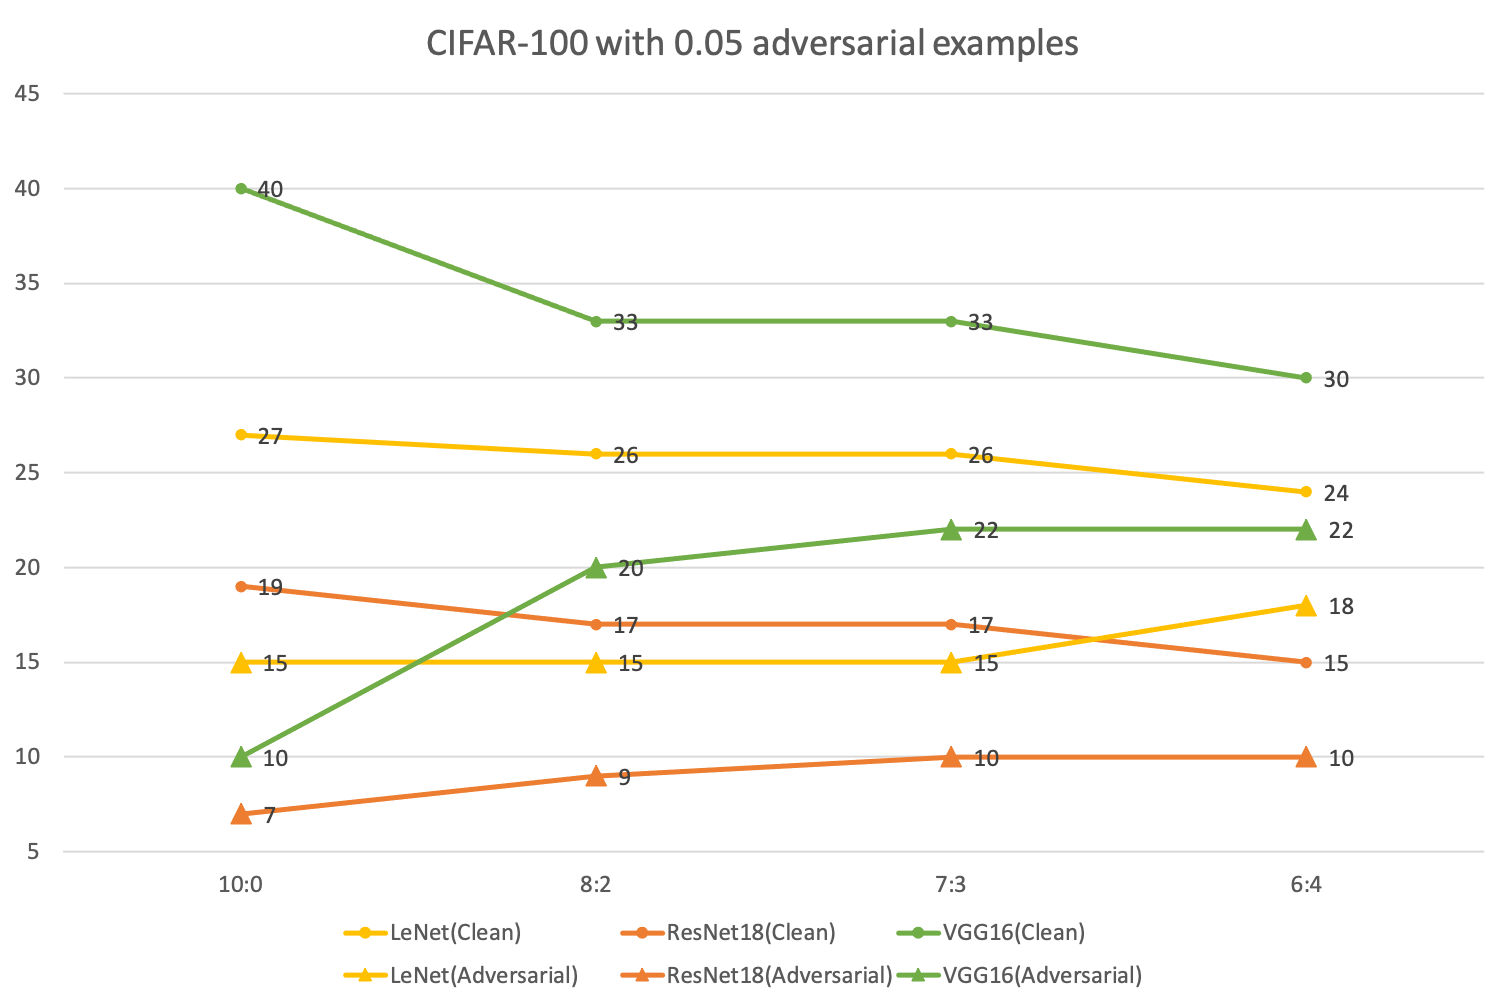
\includegraphics[width=13 cm]{Definitions/graph-005cifar100.png}
    \caption{Graphs of CIFAR-100 with \begin{math}\epsilon\end{math} of 0.05\label{cifar100-0.05-graph}}
\end{figure} 

These result are depicted in Figure~\ref{cifar100-0.05-graph} and \ref{cifar100-0.1-graph}, which graphically illustrated the Table~\ref{cifar100-results}.
Figure~\ref{cifar100-0.05-graph} shows the results for the CIFAR-100 {\it adv\_eval} with \begin{math}\epsilon\end{math} of 0.05.
In some models, the improvement in safety was smaller than the decrease in accuracy because the models were not properly trained.
However, even without proper training, safety increased by 3\%, and accuracy decreases by 2\% for the 30- and 40-model of LeNet,
whereas safety increased by 1\% and accuracy remained unchanged in the 20- and 30-model of ResNet18.

\begin{figure}[H]
    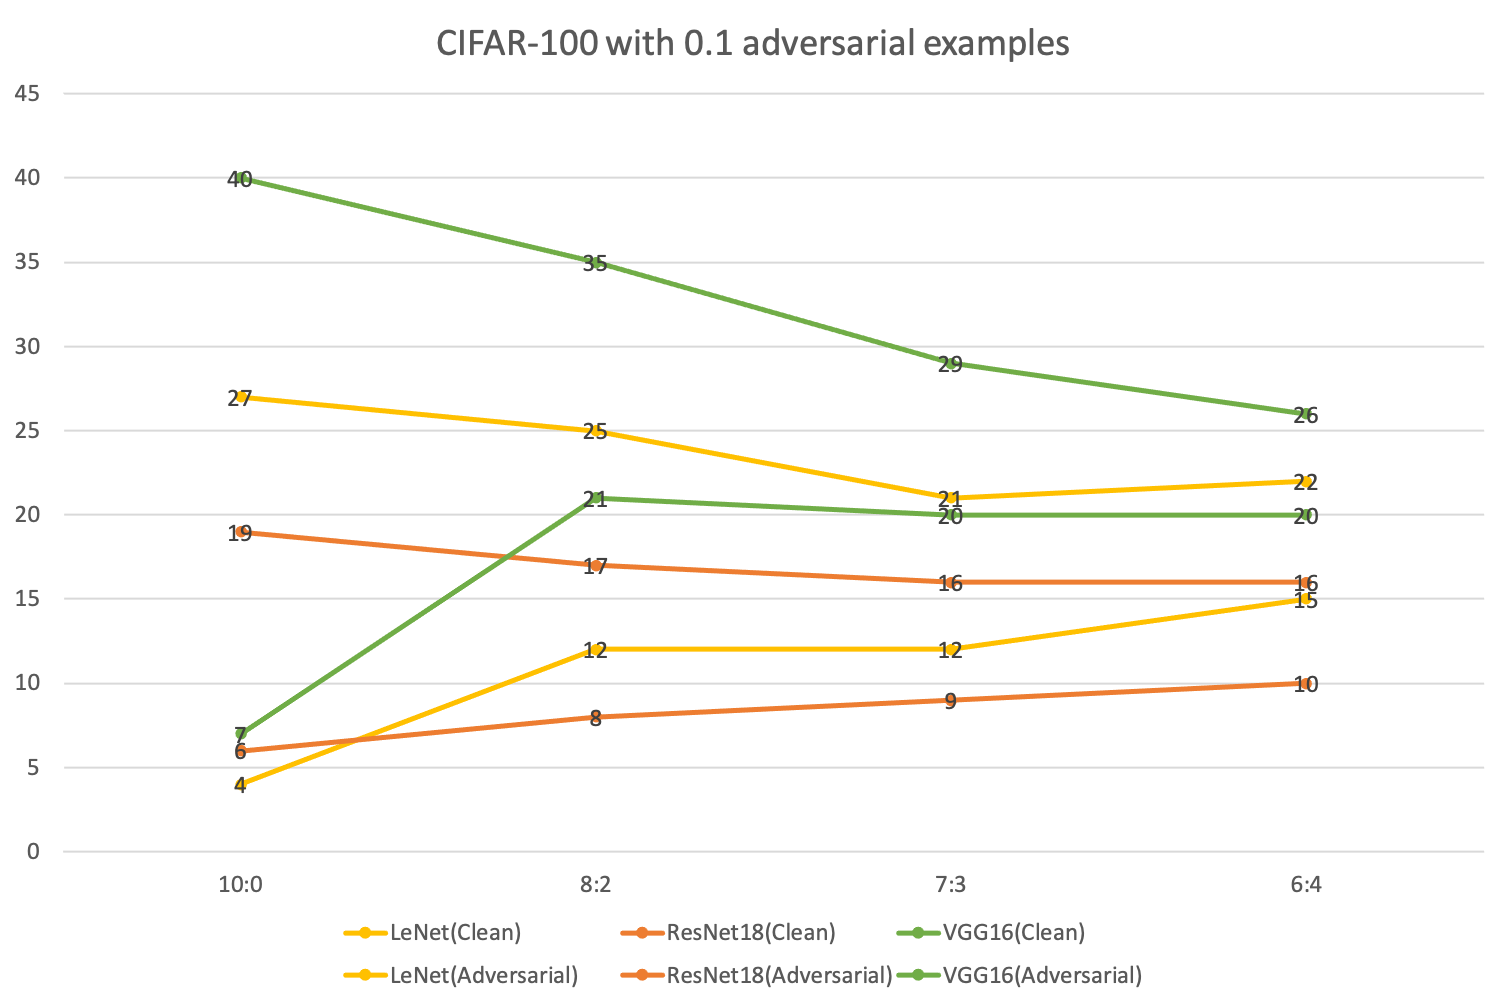
\includegraphics[width=13 cm]{Definitions/graph-01cifar100.png}
    \caption{Graphs of CIFAR-100 with \begin{math}\epsilon\end{math} of 0.1\label{cifar100-0.1-graph}}
\end{figure} 

Figure~\ref{cifar100-0.1-graph} depicts the CIFAR-100 {\it adv\_eval} results with \begin{math}\epsilon\end{math} of 0.1.
Even in ResNet18, which was not trained the most, the worst case is that where the decrease in accuracy and improvement in safety is the same;
in LeNet and VGG16, the improvement of safety was generally greater than the decrease in accuracy.
CIFAR-100 results show that adversarial training can significantly improve safety with little effect on accuracy in most, if not all cases, even for models that are not properly trained.

\subsection{GTSRB Results}

\begin{specialtable}[H]
    \centering
    \caption{Results of GTSRB with \begin{math}\epsilon\end{math}}
    \label{gtsrb-results}
    {\small
    \begin{tabular}{|c|c|c|c|c|c|c|c|c|}
    \hline
    \multirow{2}{*}{Mixed ratio} & \multirow{2}{*}{Matrix} & \multicolumn{3}{c|}{\begin{math}\epsilon=0.05\end{math}}  & \multicolumn{3}{c|}{\begin{math}\epsilon=0.1\end{math}}       \\ \cline{3-8}
                                 &                           & LeNet               & ResNet18              & VGG16       & LeNet              & ResNet18              & VGG16              \\ \hline 
    \multirow{2}{*}{10:0}        & Acc                       & 85                  & 71                    & 93          & 85                 & 71                    & 93                 \\ \cline{2-8} 
                                 & Safety                    & 17                  & 33                    & 40          & 17                 & 33                    & 40                 \\ \hline 
    \multirow{2}{*}{8:2}         & Acc                       & 76                  & 63                    & 90          & 73                 & 60                    & 85                 \\ \cline{2-8} 
                                 & Safety                    & 57                  & 49                    & 75          & 58                 & 42                    & 70                 \\ \hline 
    \multirow{2}{*}{7:3}         & Acc                       & 75                  & 60                    & 86          & 70                 & 58                    & 81                 \\ \cline{2-8} 
                                 & Safety                    & 63                  & 50                    & 76          & 65                 & 45                    & 72                 \\ \hline 
    \multirow{2}{*}{6:4}         & Acc                       & 75                  & 58                    & 87          & 65                 & 54                    & 77                 \\ \cline{2-8} 
                                 & Safety                    & 66                  & 52                    & 79          & 65                 & 46                    & 73                 \\ \hline 
    \end{tabular}
    }
\end{specialtable}

Table~\ref{gtsrb-results} shows the GTSRB results according to \begin{math}\epsilon\end{math} for each model.
The result of the 0-model shows that GTSRB exhibited the highest accuracy than the 0-model of the previous dataset but with lower safety.
The accuracy and safety significantly differ by 68\%(LeNet), 38\%(ResNet18), and 53\%(VGG16).
This confirms that the models were well trained on the original GTSRB and were vulnerable to adversarial examples.
From the previous experimental results, comparing the 0-model and 20-model, the effect of adversarial training on accuracy and safety was confirmed.
Comparing the GTSRB 0- and 20-model, we found that they were most affected by adversarial training in the used dataset.
To show this, the average of differences in accuracy and safety between 0- and 20-model for each network was calculated in each dataset.
In the case of CIFAR-10, the accuracy of LeNet and ResNet18 decreased by an average of 3\% and 2.5\%, and the safety increased by an average of 27\% and 35\%, respectively.
Also, the accuracy of VGG16 decreased by an average of 4.5\%, and the safety increased by an average of 24.5\%.
In the case of CIFAR-100, the accuracy of LeNet, ResNet18, and VGG16 decreased by an average of 1.5\%, 2\%, and 6\%, and their safety increased by an average of 4\%, 2\%, and 12\%, respectively.
In the case of GTSRB, the accuracy of the three models decreased by an average of 10.5\%, 9.5\%, and 5.5\%, and their safety increased by an average of 39.5\%, 12.5\%, and 32.5\%, respectively.
These results confirm that GTSRB also improves safety when adversarial training is performed, which is consistent with the results of other datasets.

\begin{figure}[H]
    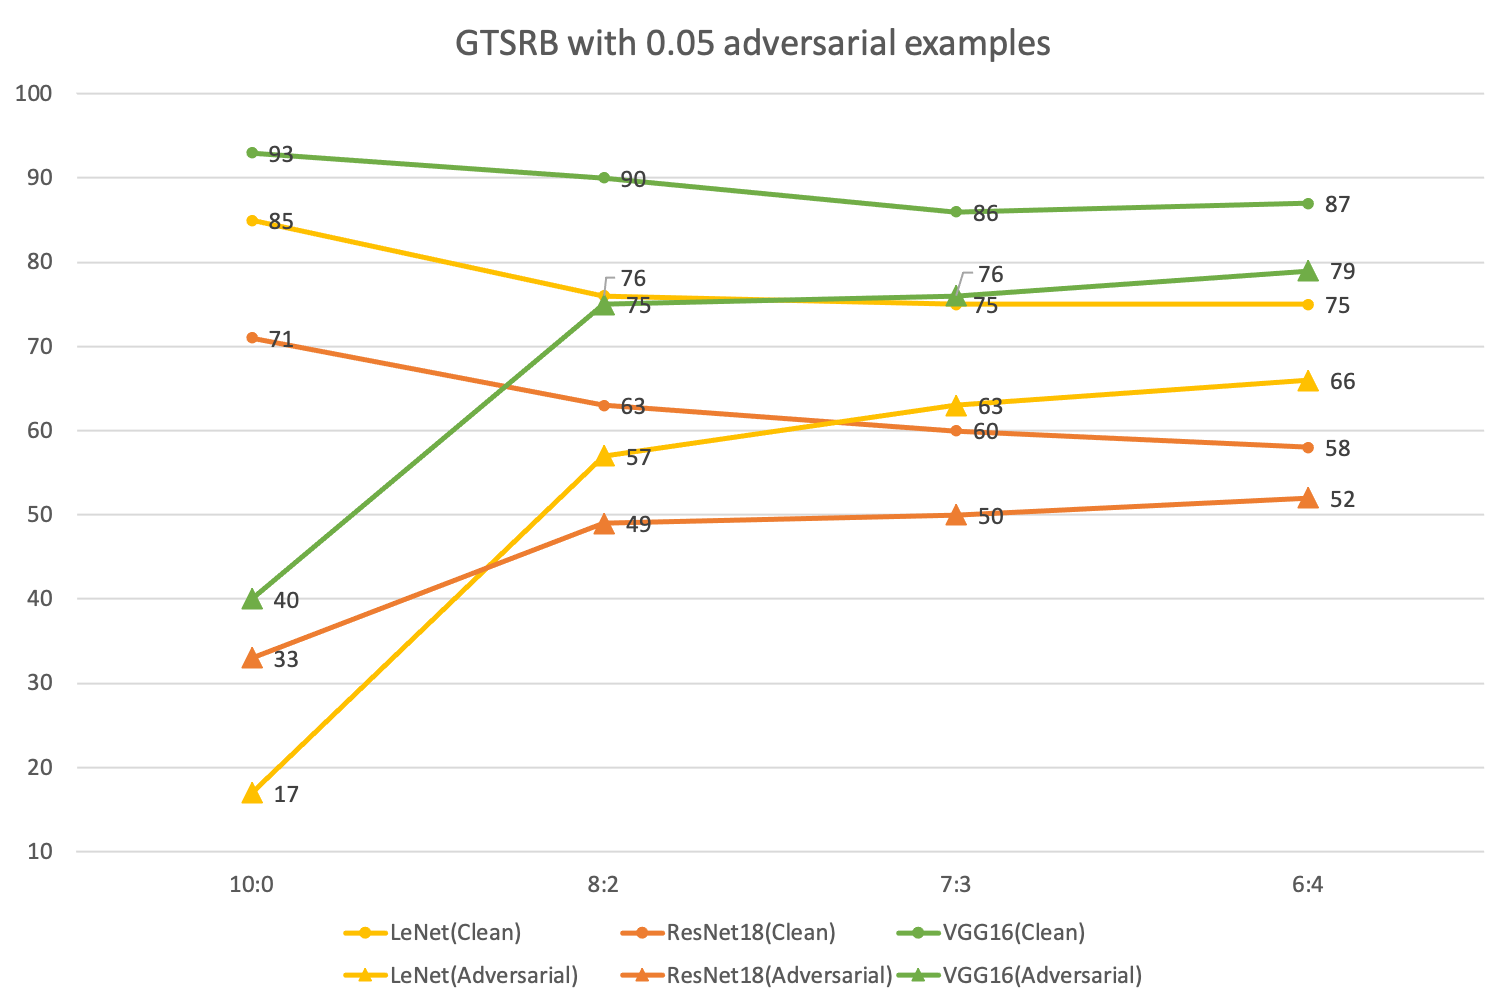
\includegraphics[width=13 cm]{Definitions/graph-005gtsrb.png}
    \caption{Graphs of GTSRB with \begin{math}\epsilon\end{math} of 0.05\label{gtsrb-0.05-graph}}
\end{figure} 

These results are depicted in Figure~\ref{gtsrb-0.05-graph} and \ref{gtsrb-0.1-graph}.
Figure~\ref{gtsrb-0.05-graph} shows the GTSRB {\it adv\_eval} results obtained with \begin{math}\epsilon\end{math} of 0.05.
In most models, except ResNet18, adversarial training could significantly improve safety with a slight decrease in accuracy.

\begin{figure}[H]
    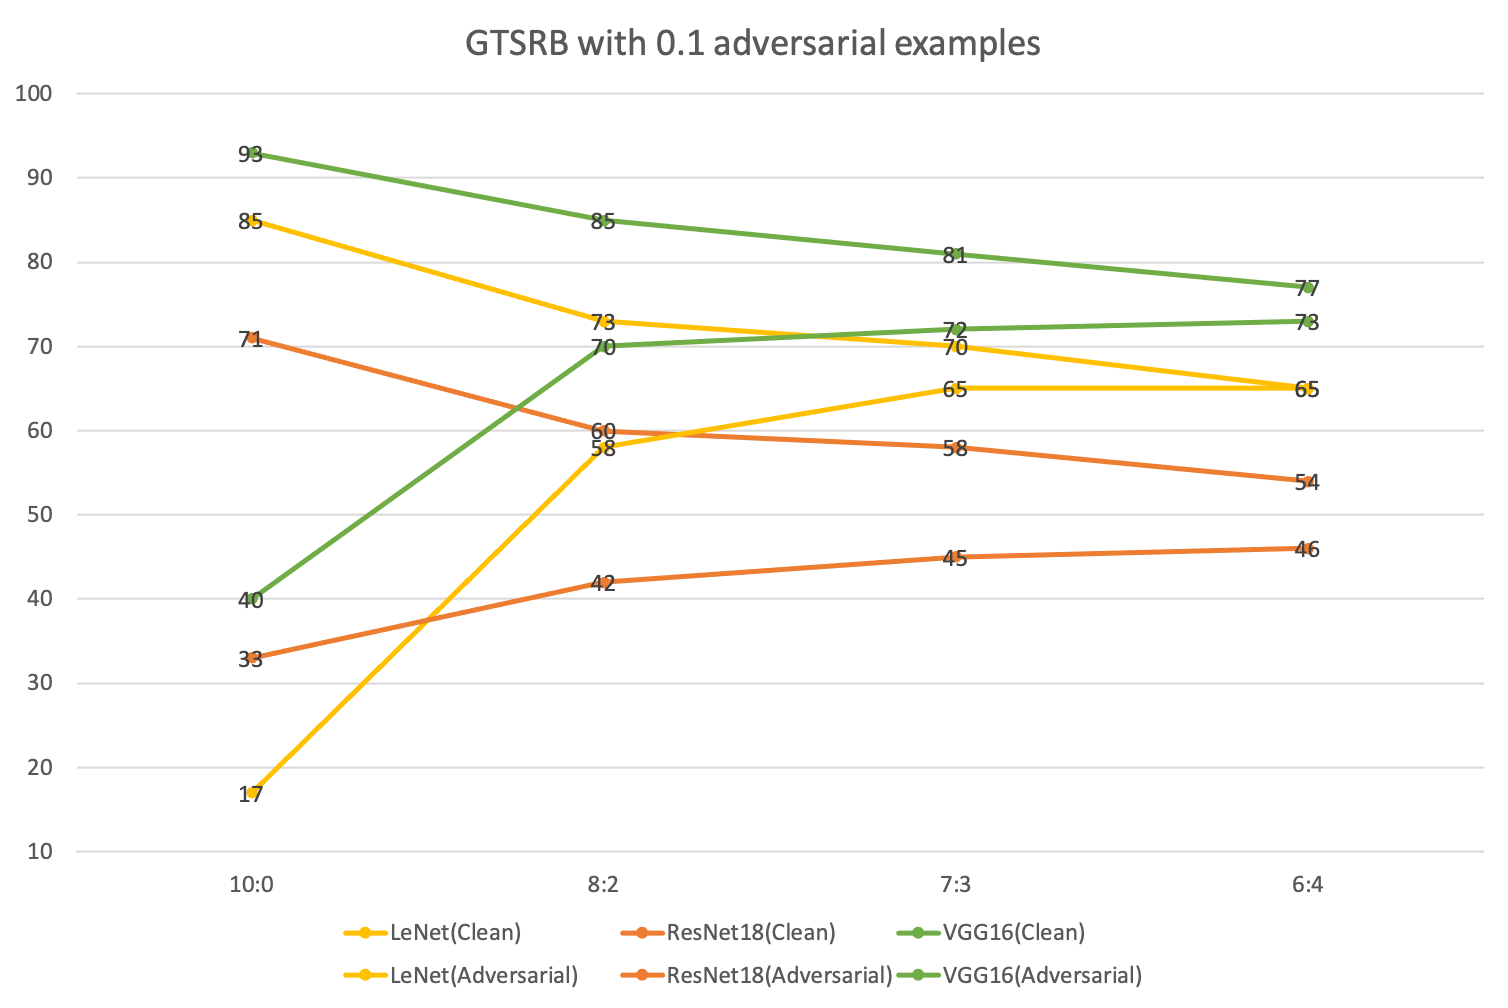
\includegraphics[width=13 cm]{Definitions/graph-01gtsrb.png}
    \caption{Graphs of GTSRB with \begin{math}\epsilon\end{math} of 0.1\label{gtsrb-0.1-graph}}
\end{figure} 

Figure~\ref{gtsrb-0.1-graph} shows the GTSRB {\it adv\_eval} results with \begin{math}\epsilon\end{math} of 0.1.
In both Figure~\ref{gtsrb-0.05-graph} and \ref{gtsrb-0.1-graph} as with the CIFAR datasets, the improvement in safety is much larger than the decrease in accuracy, and there is a slight difference among models with adversarial examples.

\subsection{Discussion}

Herein, the experimental results are discussed according to three different datasets and models and various experimental conditions, and the answer to the RQs are provided as follows.
For all datasets, the safety of 0-model has a large performance difference when compared with to the accuracy. This confirms that the adversarial examples were properly generated.

RQ1 is a question of whether adversarial training well classifies adversarial examples of classification models.
In experiments using CIFAR datasets, the safety performance of the 20-, 30-, and 40-model, including the adversarial examples, was significantly improved when compared with that of the model without adversarial examples.
This confirms that adversarial training can improve the safety performance of the classification model.
However, in CIFAR-100, training was not sufficient during the epoch, resulting in lower values, but the change in performance observed of the 0-model and other models could be observed in the similar way.

RQ2 is an extension of RQ1. It asks whether the dataset used in the experiment can have the same effect even if it is a dataset related to safety.
Although it varies, depending on the size and structure of data, GTSRB improved safety more than the CIFAR datasets.
At the same time, as in CIFAR datasets, when adversarial training was performed, the degree of improvement in safety is greater than the degree of decrease in accuracy.
This confirms that adversarial training can improve safety with a small effect on accuracy, even in safety-related datasets.

RQ3 asks whether adversarial training affects safety regardless of the structure of the model.
To prove this, in the experiment, models with three different structures were applied.
When adversarial training was performed, safety was improved when compared with the case without the training.
Although the models used in the experiment may have a greater accuracy drop when compared with the safety improvements, the overall experimental results show that they can improve safety performance without affecting accuracy, regardless of the model structure.

RQ4 is a question of what ratio would be the best performance to mix adversarial examples with original data to form a mixed training dataset.
This depends on the dataset used and whether the requirements include accuracy or safety. Herein, we considered a balance between accuracy and safety.
Experiments showed that it is essential to mix adversarial examples from the training data, at least 20\% when constructing the training dataset to verify the safety.
This is because the greatest improvement in safety could be obtained compared to the 0-model when the 20-model was used in all experimental environments.
Even when adversarial training data were included at a higher percentage, the degree of safety improvement was small. Thus, it can be considered as the minimum requirement to configure 20\% of the total training dataset as adversarial examples.
If accuracy is considered a more important requirement, the proportion of adversarial examples can be reduced, and if safety is the more important requirement, more adversarial examples can be included.

Additionally, the shape of the graphs shows the same tendency for all datasets and \begin{math}\epsilon\end{math} values.
This shows that regardless of the degree of deformation of the adversarial example, adversarial training can improve safety.

In summary, adversarial training can improve the safety of classification models, ragardless of the structure of the model, which also applies to safety-related datasets.
To verify safety, it is recommended that at least 20\% of the training data comprise adversarial examples, and the desired requirements can be verified by adjusting the inclusion ratio of adversarial examples according to priority between accuracy and safety.
On the basis of these results, we propose a new classification model training process reflecting factors that can verify safety.

\begin{figure}[H]
    
\includegraphics[width=13 cm]{Definitions/comparison.png}
    \caption{Comparison between existing processes and our process\label{comparison}}
\end{figure} 

In existing processes, the performance, one of the AI NFRs, has been verified by training the model using the original dataset and evaluating the trained model.
If the performance does not reach the standard, the same process is repeated until the set performance is achieved through finetuning processes, such as adjusting the model structure or hyperparameters or modifying the dataset.
The problem with the existing process is that it undergoes several finetuning processes to meet the desired performance standards.
It is difficult to obtain information, such as how the data should be modified and what structure the model should exhibit with simple numerical values.
Thus, it requires many resources because it is necessary to find the best optimal case by repeating the same process while changing the conditions little by little.
Herein, we propose a process that can reduce this adjustment process.
First, an adversarial dataset is created using the original dataset.
Then, using the generated adversarial dataset, a mixed training dataset is constructed, and the model is trained.
The trained model obtains accuracy and safety through the original and adversarial evaluation datasets.
Existing processes only evaluate accuracy but do not provide enough information on how to make adjustments.
However, in the proposed method, safety can be used to obtain additional information on the coordination of data by comparing priorities between accuracy and safety.
If accuracy is the more important requirement, the inclusion rate of the original data in the training dataset can be increased, and vice versa.
This does not provide information regardomg the model structure or hyperparameters finetuning but provides additional information regarding what augmentation should be applied to the minimal dataset.

%%%%%%%%%%%%%%%%%%%%%%%%%%%%%%%%%%%%%%%%%%
\section{Conclusions}

Through experiments, we found that adversarial training can improve the safety performance of models with little effect on accuracy.
This means that generating adversarial examples using the dataset obtained before proceeding with learning and including the adversarial examples in the training dataset can be applied to verify the safety of AI.
Furthermore, we propose a method to achieve a balance between accuracy and safety for the datasets used in experiments by generating a mixed dataset of different ratios.
Using the proposed method, a balance between accuracy and safety can be achieved by performing the experiment several times according to the important requirements and adjusting the ratio of inclusion of adversarial examples in the training dataset.
For an actual AI project, the proposed method can be used to verify safety before the training process, which consumes several resources by checking whether adversarial examples are included in the training dataset.
Thus, the required resources can be reduced at least for the training process.
Moreover, the cost of training models, which verify the requirements, can be reduced by adjusting the ratio of inclusion of adversarial examples for higher-value requirements through accuracy and safety after one training and evaluation.

In future studies, we shall verify the validity of the proposed method for more diverse safery-related classification datasets, different model structures, and various adversarial attack methods.
Additionally, we shall research how NFRs other than AI and safety for purposes other than classification models can be preverified through experiments.

%%%%%%%%%%%%%%%%%%%%%%%%%%%%%%%%%%%%%%%%%%
\vspace{6pt} 

%%%%%%%%%%%%%%%%%%%%%%%%%%%%%%%%%%%%%%%%%%
%% optional
%\supplementary{The following are available online at \linksupplementary{s1}, Figure S1: title, Table S1: title, Video S1: title.}

% Only for the journal Methods and Protocols:
% If you wish to submit a video article, please do so with any other supplementary material.
% \supplementary{The following are available at \linksupplementary{s1}, Figure S1: title, Table S1: title, Video S1: title. A supporting video article is available at doi: link.} 

%%%%%%%%%%%%%%%%%%%%%%%%%%%%%%%%%%%%%%%%%%
\authorcontributions{For research articles with several authors, a short paragraph specifying their individual contributions must be provided. The following statements should be used ``Conceptualization, X.X. and Y.Y.; methodology, X.X.; software, X.X.; validation, X.X., Y.Y. and Z.Z.; formal analysis, X.X.; investigation, X.X.; resources, X.X.; data curation, X.X.; writing---original draft preparation, X.X.; writing---review and editing, X.X.; visualization, X.X.; supervision, X.X.; project administration, X.X.; funding acquisition, Y.Y. All authors have read and agreed to the published version of the manuscript.'', please turn to the  \href{http://img.mdpi.org/data/contributor-role-instruction.pdf}{CRediT taxonomy} for the term explanation. Authorship must be limited to those who have contributed substantially to the work~reported.}

\funding{``This research received no external funding''}

% \institutionalreview{In this section, please add the Institutional Review Board Statement and approval number for studies involving humans or animals. Please note that the Editorial Office might ask you for further information. Please add ``The study was conducted according to the guidelines of the Declaration of Helsinki, and approved by the Institutional Review Board (or Ethics Committee) of NAME OF INSTITUTE (protocol code XXX and date of approval).'' OR ``Ethical review and approval were waived for this study, due to REASON (please provide a detailed justification).'' OR ``Not applicable'' for studies not involving humans or animals. You might also choose to exclude this statement if the study did not involve humans or animals.}

% \informedconsent{Any research article describing a study involving humans should contain this statement. Please add ``Informed consent was obtained from all subjects involved in the study.'' OR ``Patient consent was waived due to REASON (please provide a detailed justification).'' OR ``Not applicable'' for studies not involving humans. You might also choose to exclude this statement if the study did not involve humans.

% Written informed consent for publication must be obtained from participating patients who can be identified (including by the patients themselves). Please state ``Written informed consent has been obtained from the patient(s) to publish this paper'' if applicable.}

% \dataavailability{In this section, please provide details regarding where data supporting reported results can be found, including links to publicly archived datasets analyzed or generated during the study. Please refer to suggested Data Availability Statements in section ``MDPI Research Data Policies'' at \url{https://www.mdpi.com/ethics}. You might choose to exclude this statement if the study did not report any data.} 

% \acknowledgments{In this section you can acknowledge any support given which is not covered by the author contribution or funding sections. This may include administrative and technical support, or donations in kind (e.g., materials used for experiments).}

% \conflictsofinterest{Declare conflicts of interest or state ``The authors declare no conflict of interest.'' Authors must identify and declare any personal circumstances or interest that may be perceived as inappropriately influencing the representation or interpretation of reported research results. Any role of the funders in the design of the study; in the collection, analyses or interpretation of data; in the writing of the manuscript, or in the decision to publish the results must be declared in this section. If there is no role, please state ``The funders had no role in the design of the study; in the collection, analyses, or interpretation of data; in the writing of the manuscript, or in the decision to publish the~results''.} 

%%%%%%%%%%%%%%%%%%%%%%%%%%%%%%%%%%%%%%%%%%
%% Only for journal Encyclopedia
%\entrylink{The Link to this entry published on the encyclopedia platform.}

%%%%%%%%%%%%%%%%%%%%%%%%%%%%%%%%%%%%%%%%%%
%% Optional
% \appendixtitles{no} % Leave argument "no" if all appendix headings stay EMPTY (then no dot is printed after "Appendix A"). If the appendix sections contain a heading then change the argument to "yes".
% \appendixstart
% \appendix
% \section{}
% \subsection{}
% The appendix is an optional section that can contain details and data supplemental to the main text---for example, explanations of experimental details that would disrupt the flow of the main text but nonetheless remain crucial to understanding and reproducing the research shown; figures of replicates for experiments of which representative data are shown in the main text can be added here if brief, or as Supplementary Data. Mathematical proofs of results not central to the paper can be added as an appendix.

% \section{}
% All appendix sections must be cited in the main text. In the appendices, Figures, Tables, etc. should be labeled, starting with ``A''---e.g., Figure A1, Figure A2, etc. 

%%%%%%%%%%%%%%%%%%%%%%%%%%%%%%%%%%%%%%%%%%
\end{paracol}
%%%%%%%%%%%%%%%%%%%%%%%%%%%%%%%%%%%%%%%%%%
% To add notes in main text, please use \endnote{} and un-comment the codes below.
%\begin{adjustwidth}{-5.0cm}{0cm}
%\printendnotes[custom]
%\end{adjustwidth}
%%%%%%%%%%%%%%%%%%%%%%%%%%%%%%%%%%%%%%%%%%
\reftitle{References}

% Please provide either the correct journal abbreviation (e.g. according to the “List of Title Word Abbreviations” http://www.issn.org/services/online-services/access-to-the-ltwa/) or the full name of the journal.
% Citations and References in Supplementary files are permitted provided that they also appear in the reference list here. 

%=====================================
% References, variant A: external bibliography
%=====================================
%\externalbibliography{yes}
%\bibliography{your_external_BibTeX_file}

%=====================================
% References, variant B: internal bibliography
\begin{thebibliography}{999}
% NFRS - fairenss
\bibitem[Bird, S(2020)]{fairness-microsoft}
Bird, S., Dudík, M., Edgar, R., Horn, B., Lutz, R., Milan, V., Sameki, M., Wallach, H., Walker, K., Fairlearn: A toolkit for assessing and improving fairness in AI. {\em Microsoft, Tech. Rep.} {\bf 2020}, {\em MSR-TR-2020-32}; 142--149.
\bibitem[Dwork, C(2012)]{fairness-dwork}
Dwork, C., Hardt, M., Pitassi, T., Reingold, O., Zemel, R., Fairness through awareness. Proceedings of the 3rd innovations in theoretical computer science conference; pp. 214--226.
\bibitem[Feldman, M(2015)]{fairness-feldman}
Feldmen, M., Friedler, S. A., Moeller, J., Scheidegger, C., Venkatasubramanian, S., Certifying and removing disparate impact. Proceedings of the 21th ACM SIGKDD international conference on knowledge discovery and data mining; pp 259--268.
\bibitem[Tramer, F(2017)]{fairness-tramer}
Tramer, F., Atildakis, V., Geambasu, R., Hsu, D., Hubaux, J. P., Humbert, M, ..., Lin, H., Fairtest: Discovering unwarranted associations in data-driven applications. In IEEE European Symposium on SEcurity and Privacy, IEEE.
\bibitem[Zhang, J(2021)]{fairness-zhang} 
Zhang, J., Harman, M., Ignorance and Prejudice. In 2021 IEEE/ACM 43rd International Conference on Software Engineering(ICSE), IEEE.
\bibitem[Zemel, R.(2013)]{fairness-zemel}
Zemel, R., Wu, Y., Swersky, K., Pitassi, T., Dwork. C., Learning fair representations. International conference on machine learning; pp. 325--333.
% NFRS - transparency & xai
\bibitem[Yosinski, J(2015)]{transparency-yosinski}
Yosinski, J., Clune, J., Nguyen, A., Fuchs, T., Lipson, H., Understanding neural networks through deep visualization. \textit{arXiv preprint arXiv:1506.06579.}; 2015.
\bibitem[Samek, W(2017)]{xai-samek}
Samek, W., Wiegand, T., Müller, K. R., Explainable artificial intelligence: Understanding, visualizing and interpreting deep learning models. \textit{arXiv preprint arXiv:1708.08296.} 2017.
\bibitem[Arrieta, A. B.(2020)]{xai-arrieta}
Arrieta, A. B., Díaz-Rodríguez, N., Del Ser, J., Bennetot, A., Tabik, S., Barbado, A., Garcia, S., Gil-Lopez, S., Molina, D., Benjamins, R., Chatila, R., Herrera, F., Explainable Artificial Intelligence(XAI): Concepts, taxonomies, opportunities and challenges toward responsible AI. {\em Information Fusion} {\bf 2020}, {\em 58}, 82--115.
\bibitem[Ribeiro, M. T.(2016)]{xai-transparency-ribeiro}
Ribeiro, M. T., Singh, S., Guestrin, C., "Why should i trust you?" Explaining the predictions of any classifier. Proceedings of the 22nd ACM SIGKDD international conference on knowledge discovery and data mining; 1135--1144.
\bibitem[Merdoch, W. J.(2019)]{xai-transparency-murdoch}
Murdoch, W. J., Singh, C., Kumbier, K., Abbasi-Asi, R., Yu, B., Interpretable machine learning: definitions, methods, and applications. \textit{arXiv preprint arXiv:1901.04592.}; 2019.
% NFRS - security
\bibitem[Mei, S(2015)]{security-mei}
Mei, S., Zhu, X., The security of latent dirichlet allocation. Artificial Intelligence and Statistics; PMLR, 2015; pp 681--689.
\bibitem[Mei, S(2015)]{security-mei2}
Mei, S., Zhu, X., Using machine teaching to identify optimal training-set attakcs on machine learners. Twenty-Ninth AAAI Conference on Artificial Intelligence.
\bibitem[Barreno, M(2010)]{security-barreno}
Barreno, M., Nelson, B., Joseph, A. D., Tygar, J. D.,  The security of machine learning. {\em Machine Learning, 81} {\bf 2010}, {\em 2}, 121--148.
% NFRS - safety
\bibitem[Amodei, D(2016)]{safety-amodei}
Amodei, D., Olah, C., Steinhardt, J., Christiano, P., Schulman, J., Mané, D., Concrete problems in AI safety. \textit{arXiv preprint arXiv:1606.06565.}; 2016.
\bibitem[Juric, M.(2020)]{safety-juric}
Juric, M., Sandic, A., Brcic, M., AI safety: state of the field through quantitative lens. 2020 43rd International Convention on Information, Communication and Electronic Technology(MIPRO); 1254--1259.
\bibitem[Leike, J.(2017)]{safety-leike}
Leike, J., Martic, M., Krakovna, V., Ortega, P. A., Everitt, T., Lefrancq, A., ..., Legg, S., AI safety gridworlds. \textit{arXiv preprint arXiv:1711.09883.}; 2017.
% AI APPLICATIONS
\bibitem[Bojarski, M(2016)]{ai-driving-bajarski}
Bojarski, M., Del Testa, D., Dworakowski, D., Firner, B., Flepp, B., Goyal, P., ..., Zieba, K., End to end learning to self-driving cars. \textit{arXiv preprint arXiv:1604.07316.}; 2016.
\bibitem[Levinson, J(2011)]{ai-driving-levinson}
Levinson, J., Askeland, J., Becker, J., Dolson, J., Held, D., Kammel, S., ..., Thrun, S., Towards fully autonomous driving: Systems and algorithms. 2011 IEEE intelligent vehicles symposium; 163--168.
\bibitem[Fu, K(2016)]{ai-finance-fu}
Fu, K., Cheng, D., Tu, Y., Zhang, L., Credit card fraud detection using convolutional neural networks. International conference on neural information processing; Springer, Cham, 2016; pp 483-490.
\bibitem[Vieira, S(2017)]{ai-medical-vieira}
Vieira, S., Pinaya, W. H., Mechelli, A., Using deep learning to investigate the neuroimaging correlates of psychiatric and neurologicla disorders: Methods and applications. {\em Neuroscience \& Biobehavioral Reviews} {\bf 2017}, {\em 74}, 58--75.
\bibitem[Ramsundar, B(2015)]{ai-medical-ramsundar}
Ramsundar, B., Kearnes, S., Riley, P., Webster, D., Konerding, D., Pande, V., Massively multitask networks for drug discovery. \textit{arXiv preprint arXiv:1502.02072.}; 2015.
\bibitem[Holzinger, A(2017)]{ai-medical-xai-holzinger}
Holzinger, A., Biemann, C., Pattichis, C. S., Kell, D. B., What do we need to build explainable AI systems for the medical domain?. \textit{arXiv preprint arXiv:1712.09923.}; 2017.
\bibitem[Krause, J.(2016)]{ai-medical-krause}
Krause, J., Pere, A., Ng, K., Interacting with predictions: Visual inspection of black-box machine learning models. Proceedings of the 2016 CHI conference on human factors in computing systems; 5686--5697.
\bibitem[Tan, J.(2014)]{ai-medical-tan}
Tan, J., Ung, M., Cheng, C., Greence, C. S., Unsupervised feature contruction and knowledge extraction from genome-wide assays of breast cancer with denoising autoencoders. Pacific symposium on biocomputing co-charis; 132--143.
\bibitem[Pesapane, F.(2018)]{ai-medical-pesapane}
Pesapane, F., Volonté, C., Codari, M., Sardanelli, F., Artificial intelligence as a medical device in radiology: ethical and regulatory: ethical and regulatory issues in Europe and the United States. {\em Insights into imaging} {\bf 2018}, {\em 9(5)}, 743--753.
\bibitem[Miller, D. D.(2018)]{ai-medical-miller}
Miller, D. D., Brown, E. W., Artificial intelligence in medical practice: the question to the answer?. {\em The American journal of medicine} {\bf 2018}, {\em 131(2)}, 129--133.
% ADVERSARIAL TRAINING
\bibitem[Kurakin, A(2018)]{adversarial-kurakin}
Kurakin, A., Goodfellow, I., Bengio, S., Dong, Y., Liao, F., Liang, M., ..., Abe, M., Adversarial attacks and defences competition. The NIPS'17 Competition: Building Intelligent Systems; Springer, Cham, 2018; pp 195--231.
\bibitem[Szegedy, C(2013)]{adversarial-szegedy}
Szegedy, C., Zaremba, W., Sutskever, I., Bruna, J., Erhan, D., Goodfellow, I., Fergus, R., Intriguing properties of neural networks. \textit{arXiv preprint arXiv:1312.6199.}; 2013.
\bibitem[Goodfellow, I(2014)]{adversarial-goodfellow}
Goodfellow, I., Shlens, J., Szegedy, C., Explaining and harnessing adversarial examples. \textit{arXiv preprint arXiv:1412.6572.}; 2014.
\bibitem[Kurakin, A(2016)]{adversarial-kurakin2}
Kurakin, A., Goodfellow, I., Bengio, S., Adversarial examples in the physical world. \textit{arXiv preprint arXiv:1607.02533.}; 2016.
\bibitem[Papernot, N(2017)]{adversarial-papernot}
Papernot, N., McDaniel, P., Goodfellow, I., Jha, S., Celik, Z. B., Swami, A., Practical black-box attacks against machine learning. Proceedings of the 2017 ACM on Asia conference on computer and communications security; pp 506--519.
\bibitem[Yuan, X.(2019)]{adversarial-yuan}
Yuan, X., He, P., Zhu, Q., Li, X., Adversarial examples: Attacks and defenses for deep learning. {\em IEEE transactions on neural networks and learning systems} {\bf 2019}, {\em 30(9)}, 2805--2824.
% ETC
\bibitem[Paszke, A(2019)]{pytorch}
Paszke, A., Gross, S., Massa. F., Lerer, A., Bradbury, J., Channan, G., ..., Chintala, S., Pytorch: An imperative style, high performance deep leawrning library. Advances in neural information processing systems, 32; pp 8026--8037.
\bibitem[Krizhevsky, A(2009)]{cifar}
Krizhevskey, A., Hinton, G., Leawrning multiple layers of features from tiny images. 2009.
\bibitem[Stallkamp, J(2012)]{gtsrb}
Stallkamp, J., Schlipsing, M., Salmen, J., Igel, C., Man vs. computer: Benchmarking machine learning algorithms for traffic sign recognition. {\em Neural networks} {\bf 2012}, {\em 32}, 323--332.
\bibitem[LeCun, Y(1995)]{lenet}
LeCun, Y., Bottou, L., Haffner, P., Gradient-based learning applied to document recognition. Proceedings of the IEEE; 86(11); 2278--2324.
\bibitem[He, K(2016)]{resnet}
He, K., Zhang, X., Ren, S., Sun, J., Deep residual learning for image recognition. Proceedings of the IEEE conference on computer vision and pattern recognition; 770--778.
\bibitem[Simonyan, K(2014)]{vgg}
Simonyan, K., Zisserman, A., Very deep convolutional networks for large-scale image recognition. \textit{arXiv preprint arXiv:1409.1556.}; 2014.
\bibitem[Ajunwa, I(2016)]{trade-off}
Ajunwa, I., Friedler, S., Scheidegeer, C. E., Venkatasubramanian, S., Hiring by algorithm: predicting and preventing disparate impack. \textit{Available at SSRN.}; 2016.
%%%% template
% Reference 1
% \bibitem[Author1(year)]{ref-journal}
% Author~1, T. The title of the cited article. {\em Journal Abbreviation} {\bf 2008}, {\em 10}, 142--149.
% Reference 2
% \bibitem[Author2(year)]{ref-book1}
% Author~2, L. The title of the cited contribution. In {\em The Book Title}; Editor1, F., Editor2, A., Eds.; Publishing House: City, Country, 2007; pp. 32--58.
% \bibitem[Author3(year)]{ref-book2}
% Author 1, A.; Author 2, B. \textit{Book Title}, 3rd ed.; Publisher: Publisher Location, Country, 2008; pp. 154--196.
% Reference 4
% \bibitem[Author4(year)]{ref-unpublish}
% Author 1, A.B.; Author 2, C. Title of Unpublished Work. \textit{Abbreviated Journal Name} stage of publication (under review; accepted; in~press).
% Reference 5
% \bibitem[Author5(year)]{ref-communication}
% Author 1, A.B. (University, City, State, Country); Author 2, C. (Institute, City, State, Country). Personal communication, 2012.
% Reference 6
% \bibitem[Author6(year)]{ref-proceeding}
% Author 1, A.B.; Author 2, C.D.; Author 3, E.F. Title of Presentation. In Title of the Collected Work (if available), Proceedings of the Name of the Conference, Location of Conference, Country, Date of Conference; Editor 1, Editor 2, Eds. (if available); Publisher: City, Country, Year (if available); Abstract Number (optional), Pagination (optional).
% Reference 7
% \bibitem[Author7(year)]{ref-thesis}
% Author 1, A.B. Title of Thesis. Level of Thesis, Degree-Granting University, Location of University, Date of Completion.
% Reference 8
% \bibitem[Author8(year)]{ref-url}
% Title of Site. Available online: URL (accessed on Day Month Year).
\end{thebibliography}

% If authors have biography, please use the format below
%\section*{Short Biography of Authors}
%\bio
%{\raisebox{-0.35cm}{\includegraphics[width=3.5cm,height=5.3cm,clip,keepaspectratio]{Definitions/author1.pdf}}}
%{\textbf{Firstname Lastname} Biography of first author}
%
%\bio
%{\raisebox{-0.35cm}{\includegraphics[width=3.5cm,height=5.3cm,clip,keepaspectratio]{Definitions/author2.jpg}}}
%{\textbf{Firstname Lastname} Biography of second author}

% The following MDPI journals use author-date citation: Admsci,  Arts, Econometrics, Economies, Genealogy, Humanities, IJFS, Jintelligence, JRFM, Languages, Laws, Literature, Religions, Risks, Social Sciences. For those journals, please follow the formatting guidelines on http://www.mdpi.com/authors/references
% To cite two works by the same author: \citeauthor{ref-journal-1a} (\citeyear{ref-journal-1a}, \citeyear{ref-journal-1b}). This produces: Whittaker (1967, 1975)
% To cite two works by the same author with specific pages: \citeauthor{ref-journal-3a} (\citeyear{ref-journal-3a}, p. 328; \citeyear{ref-journal-3b}, p.475). This produces: Wong (1999, p. 328; 2000, p. 475)

%%%%%%%%%%%%%%%%%%%%%%%%%%%%%%%%%%%%%%%%%%
%% for journal Sci
%\reviewreports{\\
%Reviewer 1 comments and authors’ response\\
%Reviewer 2 comments and authors’ response\\
%Reviewer 3 comments and authors’ response
%}
%%%%%%%%%%%%%%%%%%%%%%%%%%%%%%%%%%%%%%%%%%
\end{document}

